\PassOptionsToPackage{unicode=true}{hyperref} % options for packages loaded elsewhere
\PassOptionsToPackage{hyphens}{url}
%
\documentclass[]{article}
\usepackage{lmodern}
\usepackage{amssymb,amsmath}
\usepackage{ifxetex,ifluatex}
\usepackage{fixltx2e} % provides \textsubscript
\ifnum 0\ifxetex 1\fi\ifluatex 1\fi=0 % if pdftex
  \usepackage[T1]{fontenc}
  \usepackage[utf8]{inputenc}
  \usepackage{textcomp} % provides euro and other symbols
\else % if luatex or xelatex
  \usepackage{unicode-math}
  \defaultfontfeatures{Ligatures=TeX,Scale=MatchLowercase}
\fi
% use upquote if available, for straight quotes in verbatim environments
\IfFileExists{upquote.sty}{\usepackage{upquote}}{}
% use microtype if available
\IfFileExists{microtype.sty}{%
\usepackage[]{microtype}
\UseMicrotypeSet[protrusion]{basicmath} % disable protrusion for tt fonts
}{}
\IfFileExists{parskip.sty}{%
\usepackage{parskip}
}{% else
\setlength{\parindent}{0pt}
\setlength{\parskip}{6pt plus 2pt minus 1pt}
}
\usepackage{hyperref}
\usepackage{xcolor}
%\hypersetup{
%           pdfborder={0 0 0},
%           breaklinks=true}
\hypersetup{
    colorlinks,
    linkcolor={red!50!black},
    citecolor={blue!50!black},
    urlcolor={blue!80!black}
}
\urlstyle{same}  % don't use monospace font for urls
\usepackage{graphicx,grffile}
\makeatletter
\def\maxwidth{\ifdim\Gin@nat@width>\linewidth\linewidth\else\Gin@nat@width\fi}
\def\maxheight{\ifdim\Gin@nat@height>\textheight\textheight\else\Gin@nat@height\fi}
\makeatother
% Scale images if necessary, so that they will not overflow the page
% margins by default, and it is still possible to overwrite the defaults
% using explicit options in \includegraphics[width=0.75\linewidth][width, height, ...]{}
\setkeys{Gin}{width=\maxwidth,height=\maxheight,keepaspectratio}
\setlength{\emergencystretch}{3em}  % prevent overfull lines
\providecommand{\tightlist}{%
  \setlength{\itemsep}{0pt}\setlength{\parskip}{0pt}}
\setcounter{secnumdepth}{0}
% Redefines (sub)paragraphs to behave more like sections
\ifx\paragraph\undefined\else
\let\oldparagraph\paragraph
\renewcommand{\paragraph}[1]{\oldparagraph{#1}\mbox{}}
\fi
\ifx\subparagraph\undefined\else
\let\oldsubparagraph\subparagraph
\renewcommand{\subparagraph}[1]{\oldsubparagraph{#1}\mbox{}}
\fi

% set default figure placement to htbp
\makeatletter
\def\fps@figure{htbp}
\makeatother


%\date{}

\begin{document}

\title{ZSS: Zipper logic revisited}

\author{Marius Buliga \\ \href{https://mbuliga.github.io}{mbuliga.github.io}}

\date{09.06.2021}

\maketitle

\begin{abstract}
Can we compute with tangles and Reidemeister moves? I explain where this problem comes from, why it is different than the usual way of using tangles in computation and then I propose the Zip-Slip-Smash (ZSS) graph rewriting system, which is  an improvement of zipper logic arXiv:1405.6095, and prove that it allows universal computation
using tangles and zippers, via directed Interaction Combinators.
\end{abstract}

%Buliga, Marius (2021): ZSS: Zipper logic revisited. figshare.  https://doi.org/10.6084/m9.figshare.14769666.v1 


\hypertarget{introduction}{%
\section{Introduction}\label{zss-zipper-logic-revisited}}



This is based on the transcript of a talk from September 2020, which I
gave at the
\href{https://www.dropbox.com/sh/5c3xihm2mkdo5s5/AADl_aRwAB3EfT2YpiLfCRZ-a?dl=0}{Quantum
Topology Seminar} organized by Louis Kauffman.

There is a
\href{https://www.dropbox.com/sh/5c3xihm2mkdo5s5/AABDoNpc6K4XioJqesIy6vdma/MariusBuliga?dl=0\&preview=zoom_0.mp4\&subfolder_nav_tracking=1}{video
of the talk} and a \href{https://github.com/mbuliga/zss}{github
repository} associated with ZSS.

\textbf{The problem:} is to compute with Reidemeister moves, i.e by use of a graph
rewrite system which contains the tangle diagrams as graphs and
Reidemeister moves as graph rewrites.

Can we do universal computation with this?

\hypertarget{where-does-this-problem-come-from}{%
\subsection{Where does this problem come
from?}\label{where-does-this-problem-come-from}}

This is not the usual way to do computation with tangles. The usual way, Figure \ref{usual-use-of-R-moves}, 
is that we have a circuit which we represent as a tangle, a knot
diagram, where the crossings and maybe caps and cups are operators which
satisfy the algebraic equivalent of the R moves.

\begin{figure}[h!]
\centering
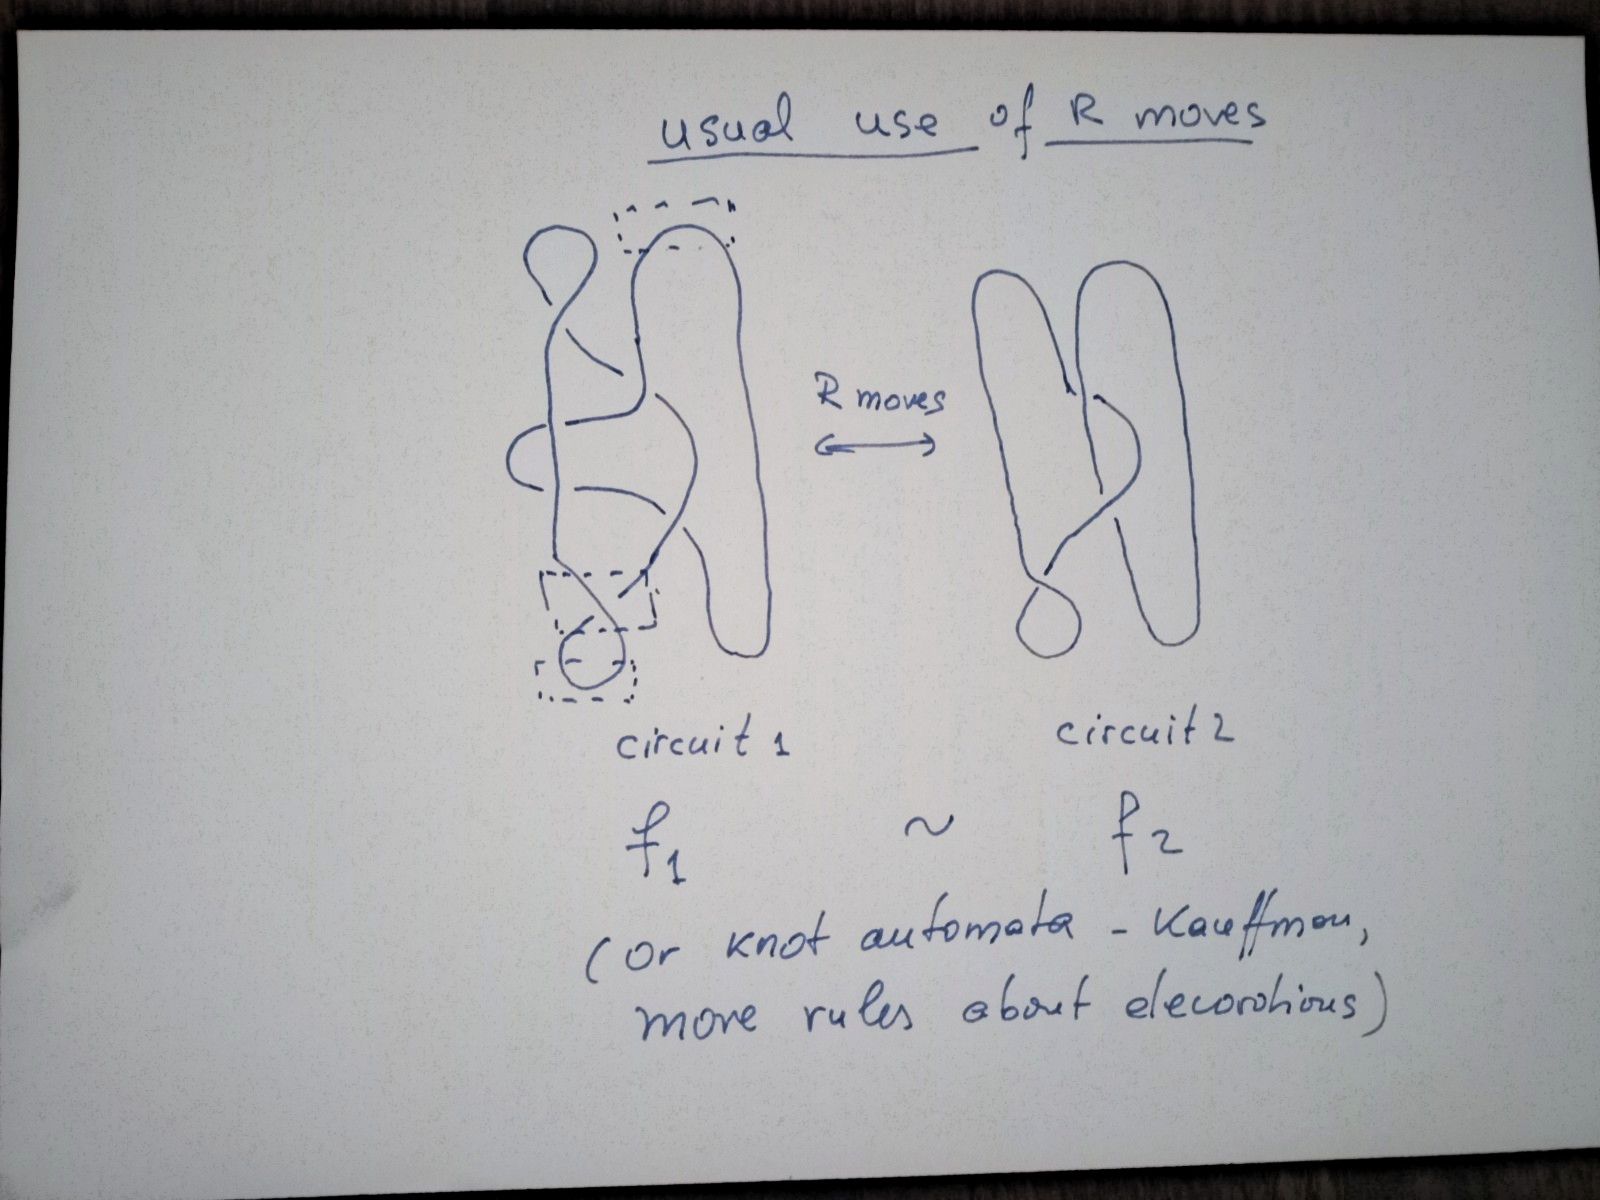
\includegraphics[width=0.75\linewidth]{img/2818.jpg}
\caption{usual use of R moves}
\label{usual-use-of-R-moves}
\end{figure}

Each circuit represents a computation. When we have two circuits, then
we can say that they represent equivalent computations when we can turn
one into another by using R moves.

As an example, in graphical formalisms used for quantum computation
\href{https://arxiv.org/pdf/0906.4725.pdf}{like ZX calculus} \cite{zx} we have
preparation (cups), detectors (caps) and crossings are quantum gates. R
moves and cup-cap annihilation graph rewrites transform a computation
into another. The well known example of teleportation shows that two
computation are equivalent. The first computation has associated a graph
which represents the teleportation experiment. It is not clear what is
the effect of this computation. The second computation is obviously
clear to us (teleportation) but it is not clear how we can realize this
computation in practice. The equivalence (not via R moves in this case,
but involving the annihilation of a cup with a cap) between the two
graphs show that these two graphs represent the same computation,
therefore we obtain an explanation why the experimental setting achieves
the effect of teleportation.

We see here that the graph rewrites don't compute by themselves, instead
they are used to prove that two computations are equivalent. The graph
rewrites do not compute!

My source of interest in the problem if we can compute with the R moves
comes from emergent algebras, introduced in \cite{buligairq} 
\href{http://arxiv.org/abs/0907.1520}{arXiv:0907.1520} and their
graphical representations using tangles \cite{buligatangle}
\href{http://arxiv.org/abs/1103.6007}{arXiv:1103.6007}. An e.a. is a
combination of algebraic and topological information, see Figure \ref{definition-of-emergent-algebras}.

\begin{figure}[h!]
\centering
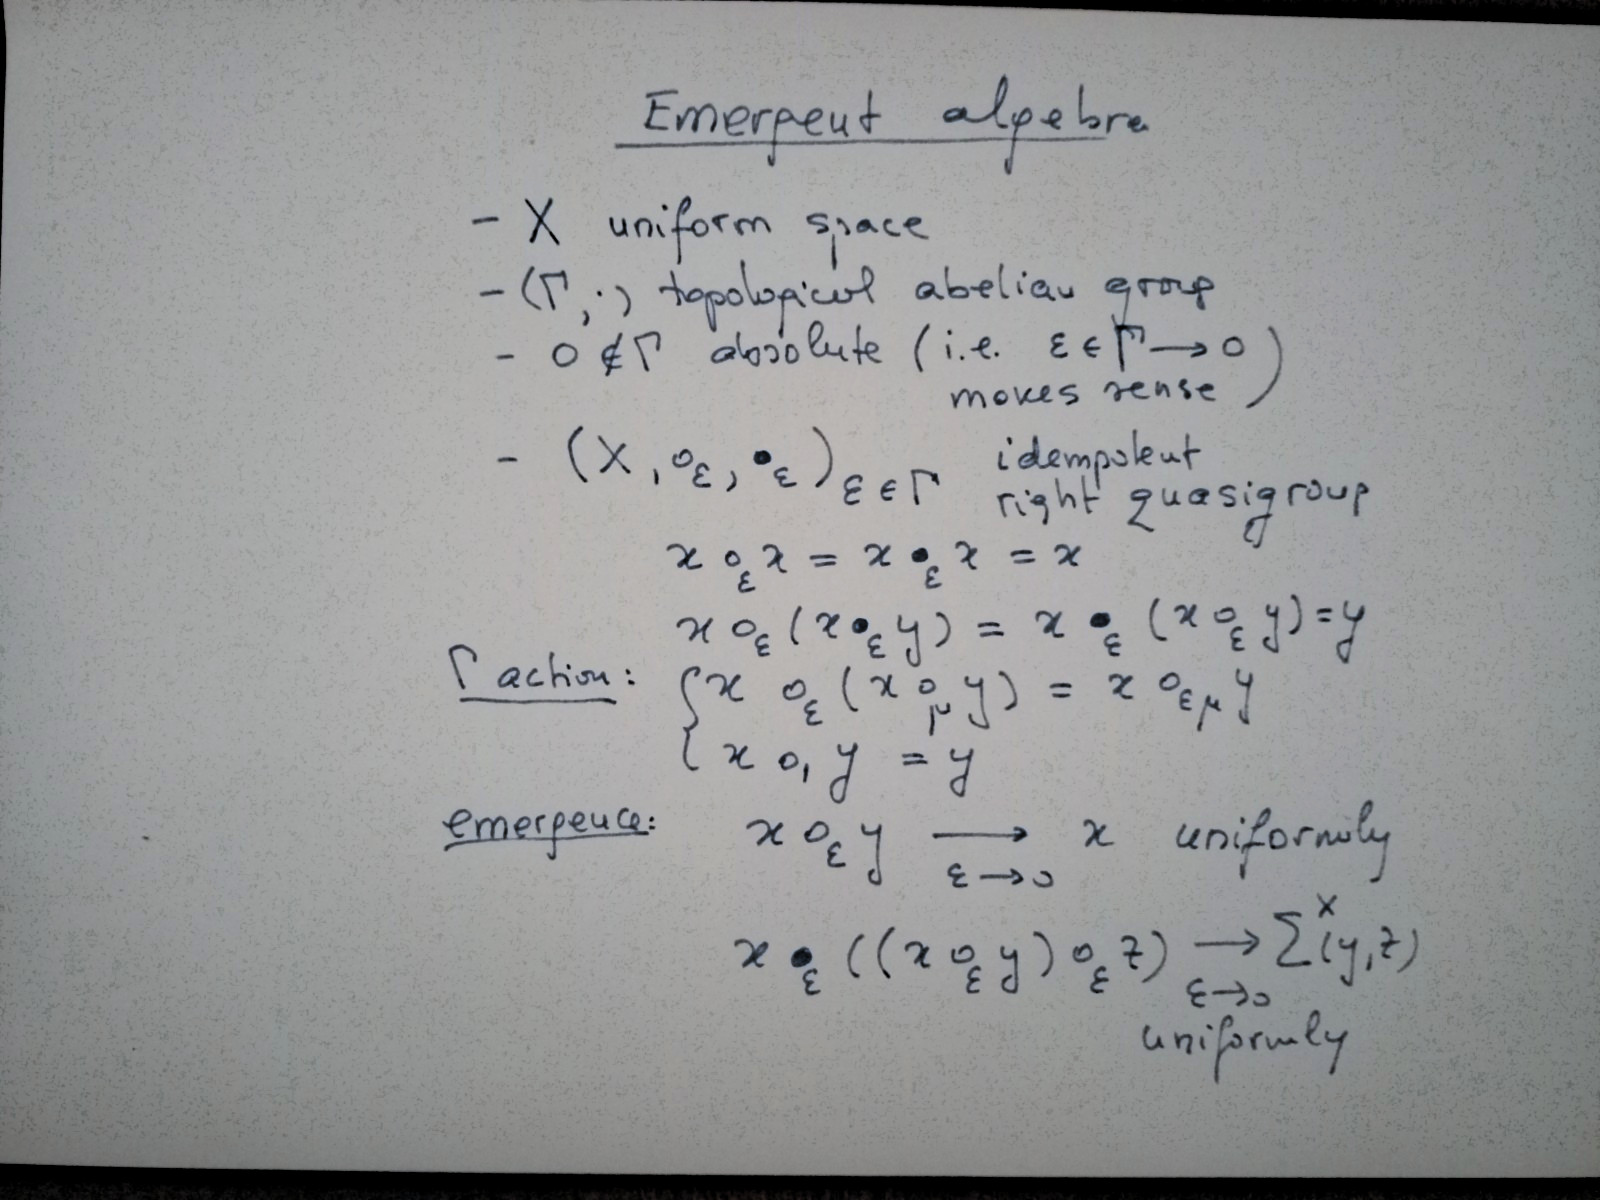
\includegraphics[width=0.75\linewidth]{img/2626.jpg}
\caption{definition of emergent algebras}
\label{definition-of-emergent-algebras}
\end{figure}

See also  \cite{buligaem} 
\href{https://arxiv.org/abs/1807.02058}{arXiv:1807.02058} for an
associated lambda calculus style term rewriting system.

For convenience, I reproduce here the short description of emergent algebras from \cite{buligacolin} \href{https://mbuliga.github.io/colin/colin.pdf}{A problem in
emergent algebras}. 

{\bf Definition.} An emergent algebra over a set $X$ is a family of idempotent left quasigroup operations over X, 
indexed by the group $\Gamma$, which satisfy the following algebraic and topological axioms (R1), (R2), (act) and (em). \\


For $a \in \Gamma$ let's denote the left quasigroup operations indexed by $a$ with $\circ_a$ and $\bullet_a$. Therefore 
$(X,\circ_a ,\bullet_a )$ is an idempotent left quasigroup: \\

\paragraph{(R1)} $x \circ_a x = x$ 
 
\paragraph{(R2)} $x \circ_a (x \bullet_a y) = x \bullet_a (x \circ_a y) = y$ \\
   


\paragraph{(act)} algebraic axioms which relate the operations: \\

      $x \circ_a ( x \circ_b y) = x \circ_{ab} y $
      
      $x \circ_1 y = y $
      
      $x \circ_{1/a} y = x \bullet_a y $\\


\noindent On $X$ we define the following operations which we will use later:\\ 

- the approximate difference \\  

$\Delta^{x}_{a} (y , z)  =  (x \circ_a y) \bullet_a (x \circ_a z) $\\ 

- the approximate sum \\  

$\Sigma^{x}_{a} (y, z) = x \bullet_{a} ( ( x \circ_{a} y) \circ_{a} z)$  \\ 

- the approximate inverse \\

$inv^{x}_{a} y = (x \circ_{a} y) \bullet_{a} x$ \\

\noindent Finally we have the topological axioms. 


\paragraph{(em)} $X$ is an uniform space; as $a$ converges to $0$ \\

     $(x,y) \mapsto x \circ_a y$ converges uniformly to  $(x,y) \mapsto x$  

     $(x,y,z) \mapsto \Delta^{x}_{a} (y , z)$ converges uniformly to a function $(x,y,z) \mapsto \Delta^{x} (y , z)$

      $(x,y,z) \mapsto \Sigma^{x}_{a} (y , z)$ converges uniformly to a function $(x,y,z) \mapsto \Sigma^{x} (y , z)$ \\


\vspace{.5cm}

By the usual correspondence between quandles and crossings, in emergent
algebras we can perform the Reidemeister 1 and 2 moves, but not the R3.
On the other hand, we can pass to the limit with the parameter which
decorates the operations (or crossings).

This passage to the limit produces emergent objects and properties. Here
is how.

In Figure \ref{emergent-sum} is the configuration which gives the approximate sum.

\begin{figure}[h!]
\centering
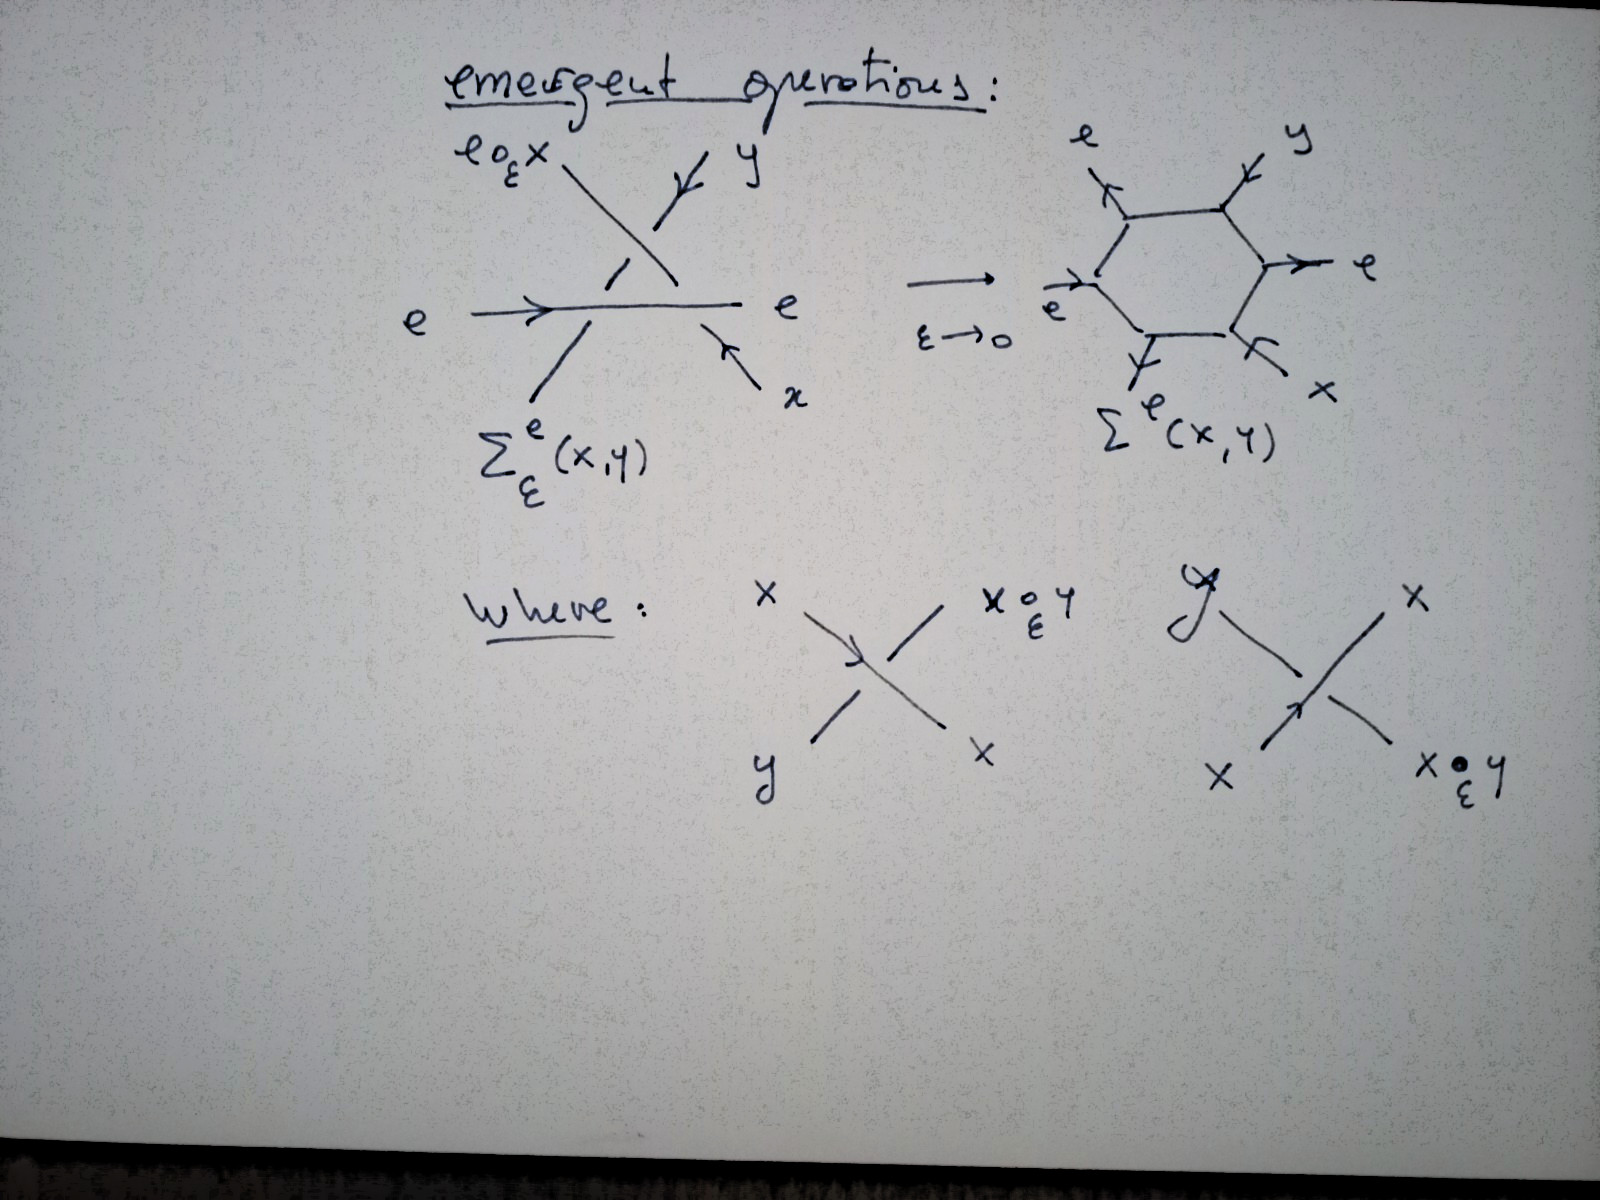
\includegraphics[width=0.75\linewidth]{img/2644.jpg}
\caption{emergent sum}
\label{emergent-sum}
\end{figure}

The crossings represent emergent algebra operations. The graphical
representation tells that as epsilon goes to 0 you obtain in the limit
some gate (the sum gate, drawn as a hexagon) which has 3 inputs and 3
outputs.

We say that the sum is an emergent object because it emerges from the
limit. We can also define in the same way the derivative of a function,
graphically, as in Figure \ref{definition-of-the-derivative}.

\begin{figure}[h!]
\centering
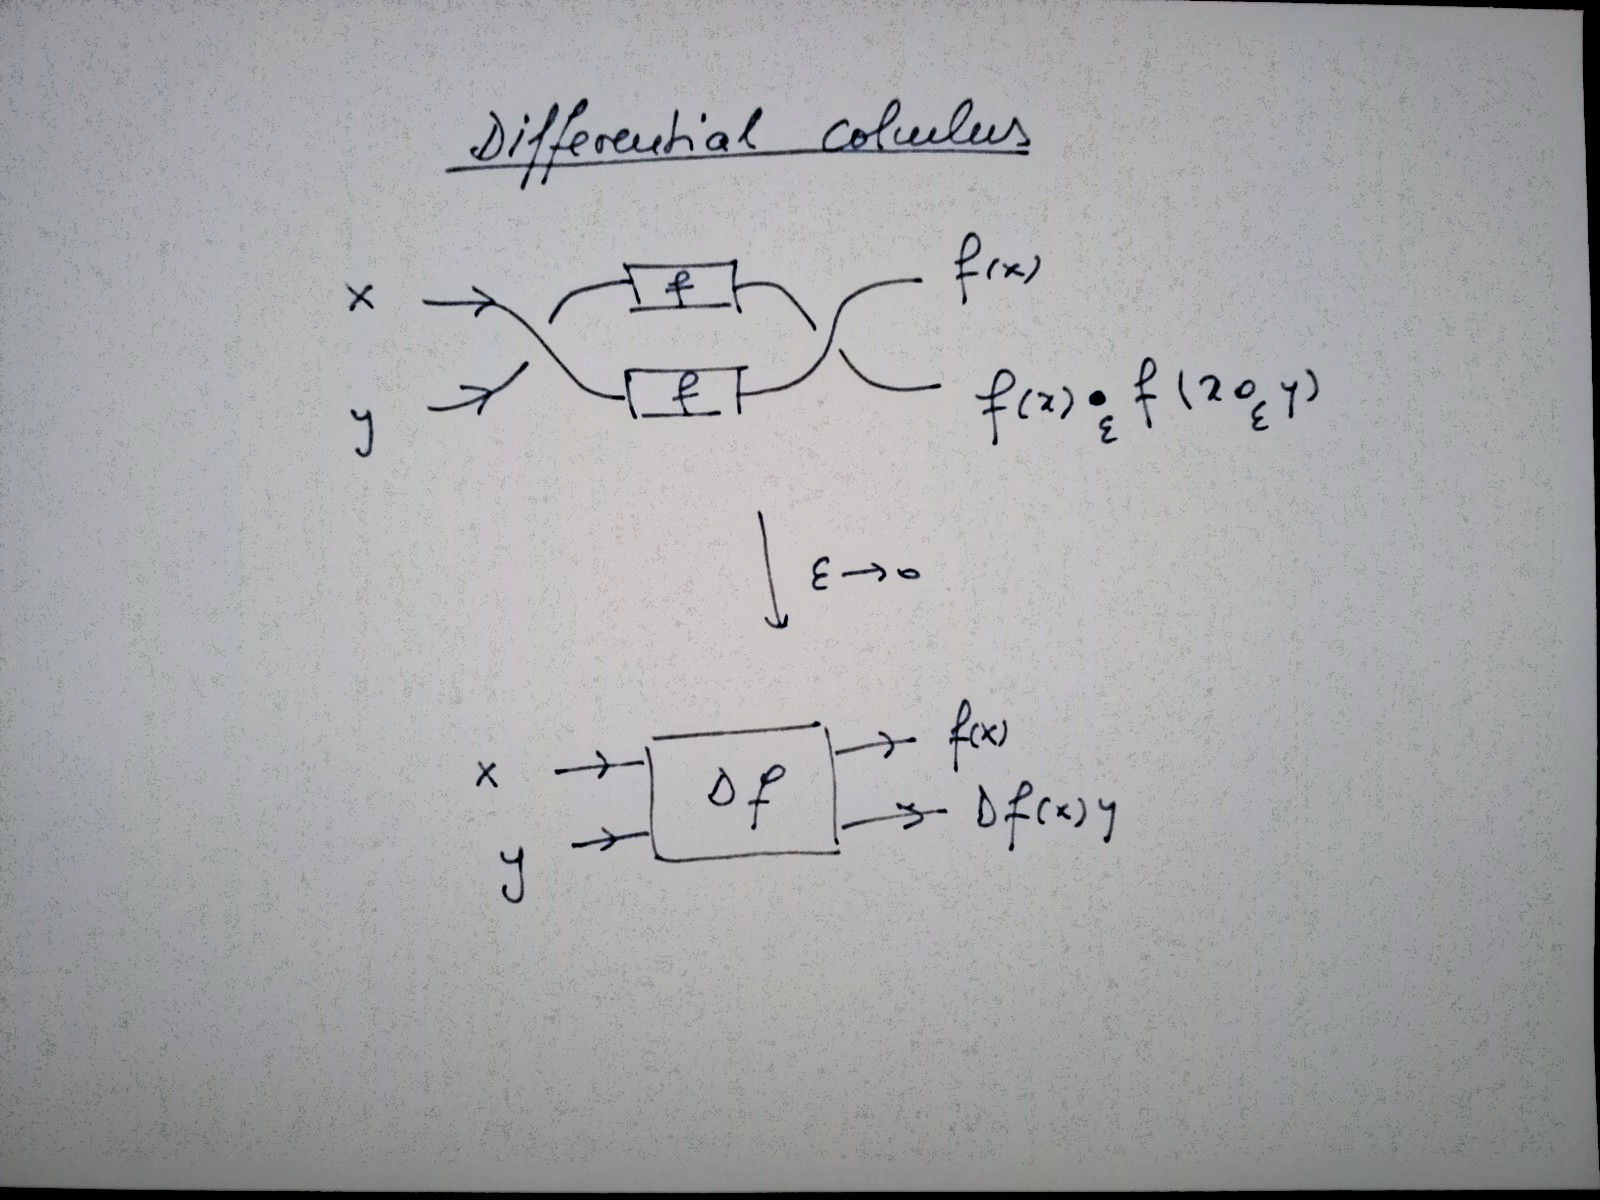
\includegraphics[width=0.75\linewidth]{img/2701.jpg}
\caption{definition of the derivative}
\label{definition-of-the-derivative}
\end{figure}

We can define not only emergent objects, but also emergent properties.

As an example, in Figure \ref{associativity-as-emergent-property} we use the R2 rewrites and passage to the limit
to prove that the addition is associative.

\begin{figure}[h!]
\centering
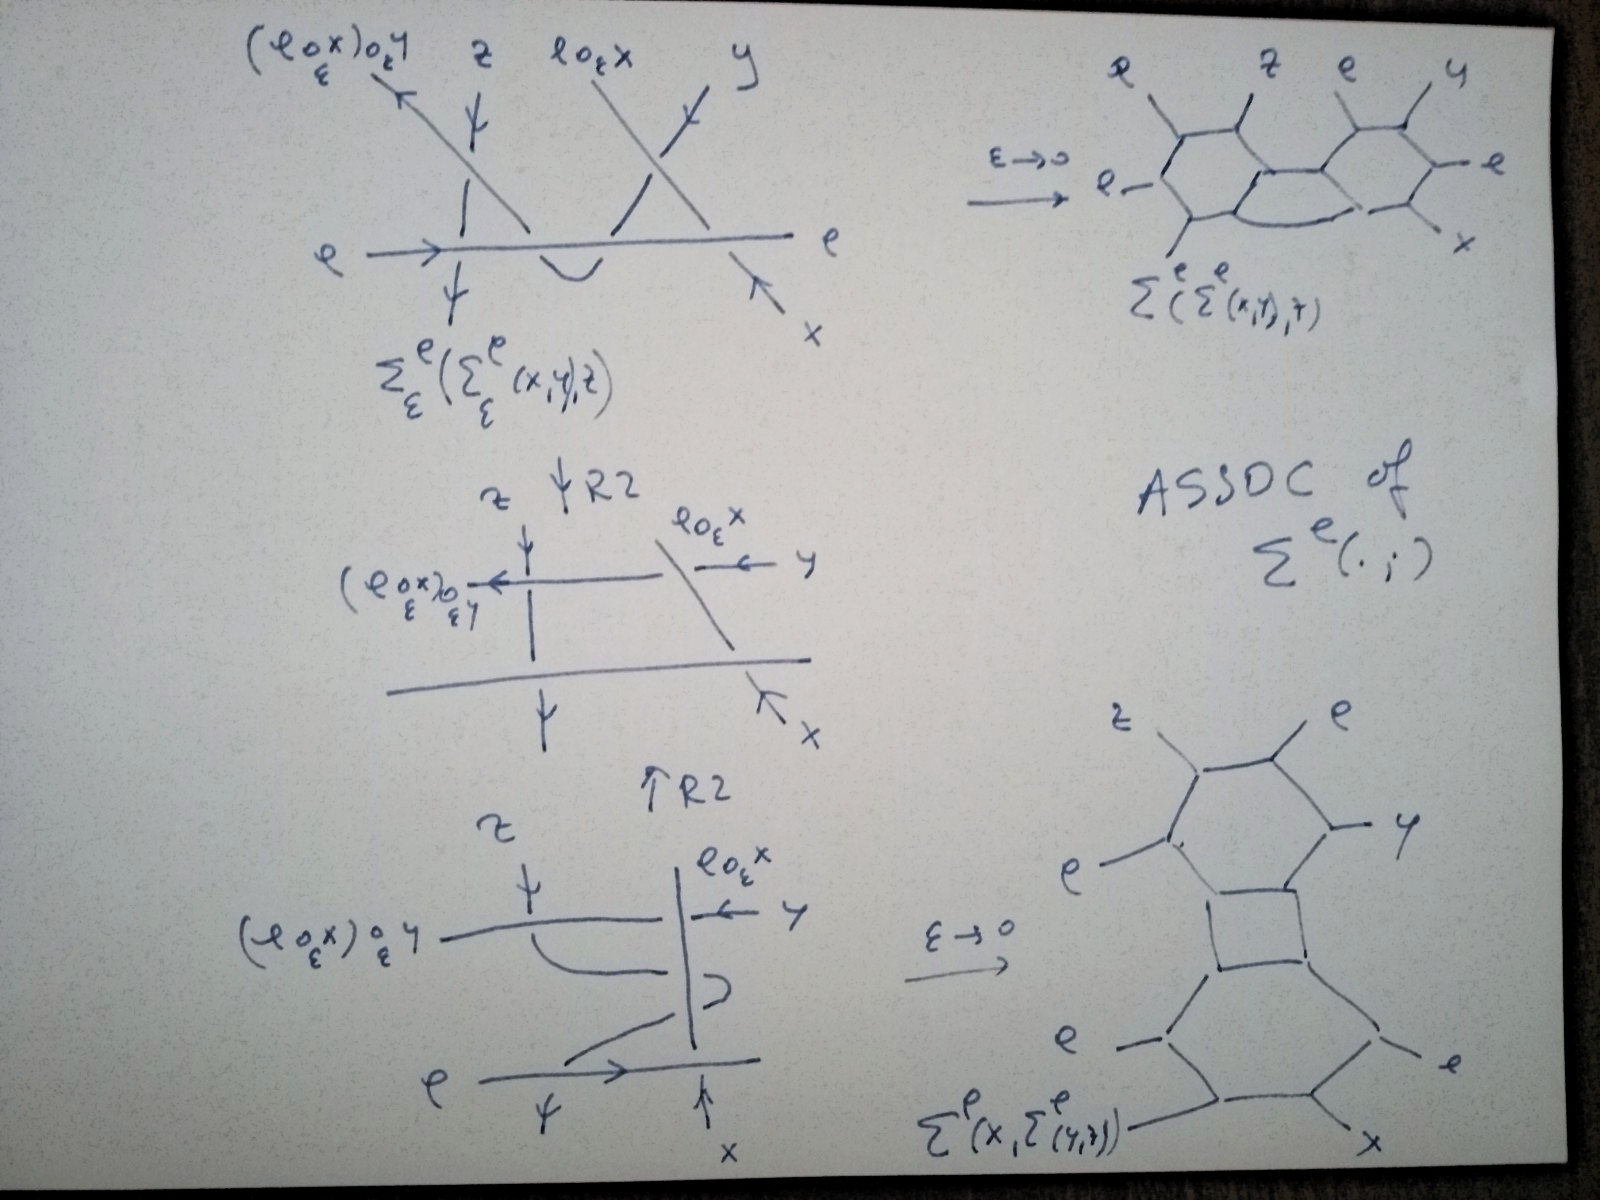
\includegraphics[width=0.75\linewidth]{img/2715.jpg}
\caption{associativity as emergent property}
\label{associativity-as-emergent-property}
\end{figure}

The mechanism is: you pass to the limit from left to right of the figure and
you use R2 rewrites from up to down, to obtain the associativity of the
sum operation in graphical form.

Another example in Figure \ref{R3-emerges-from-R1-and-R2}: if you define a new crossing (relative crossing) then
you can pass to the limit and you can prove that, based on e.a. axioms,
including a passage to the limit, the R3 emerges.

\begin{figure}[h!]
\centering
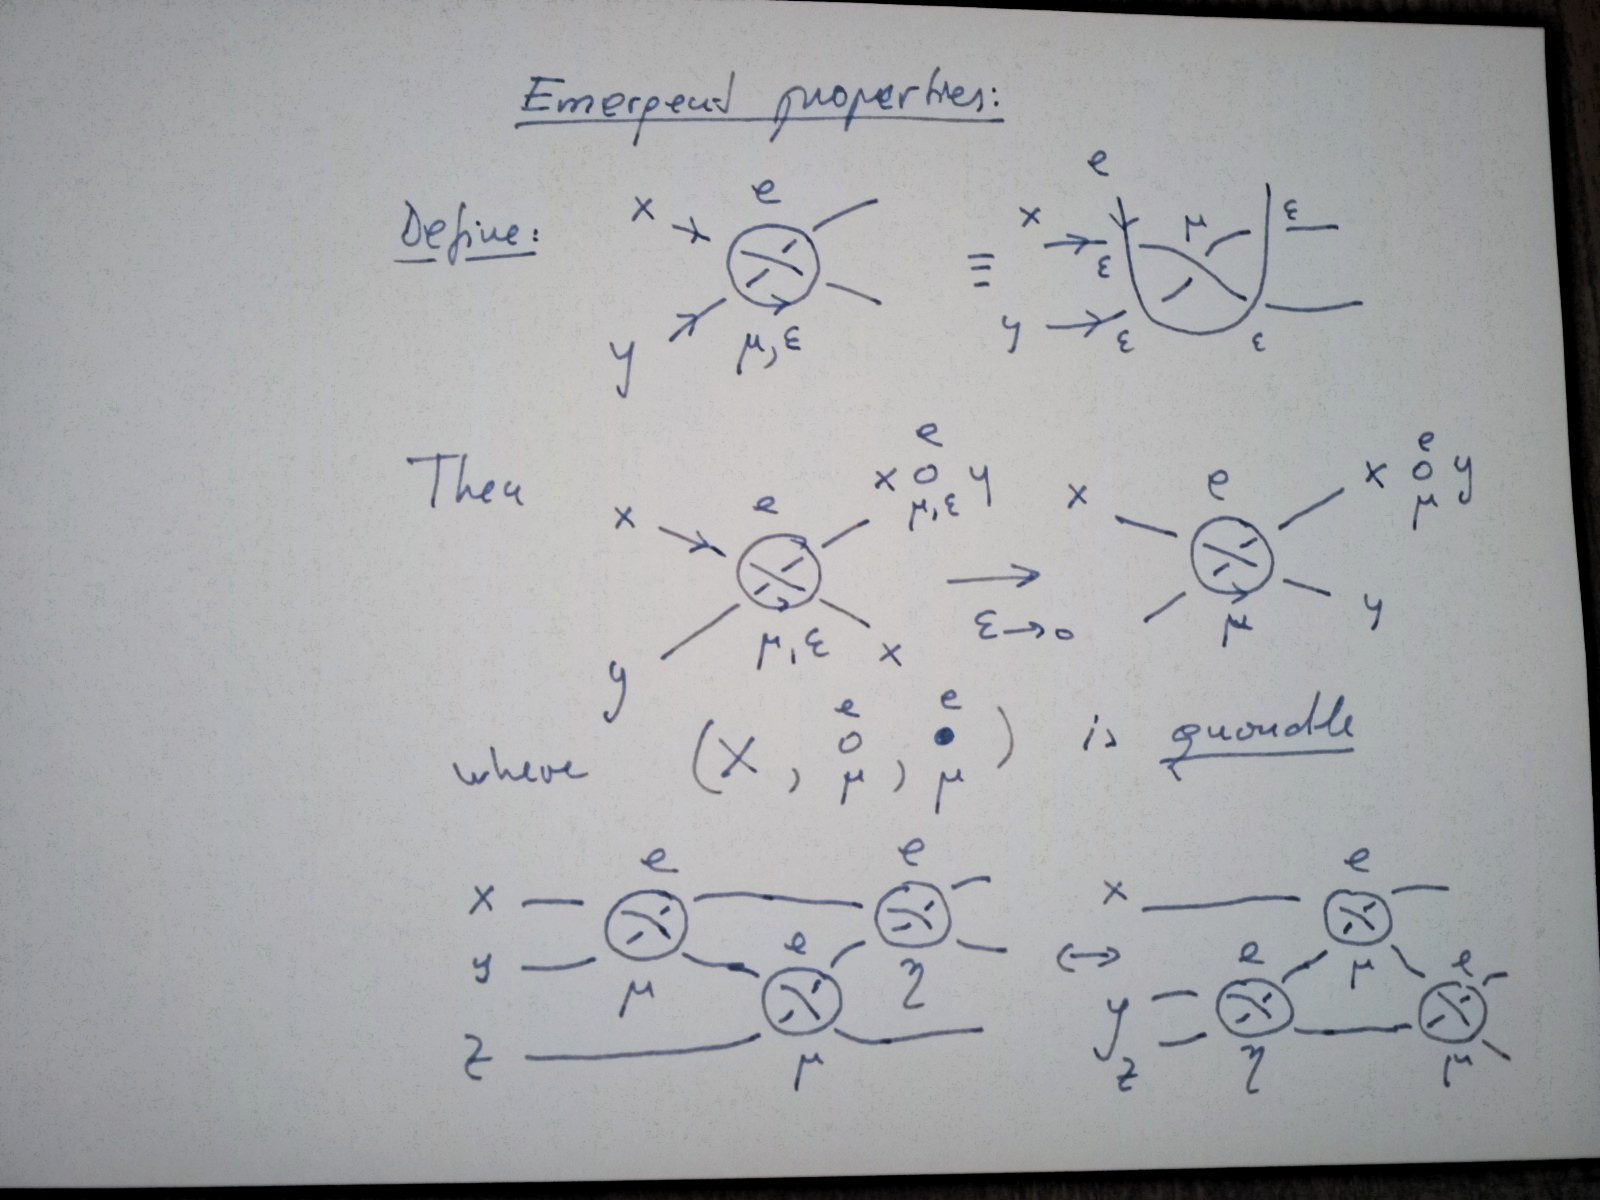
\includegraphics[width=0.75\linewidth]{img/2734.jpg}
\caption{R3 emerges from R1 and R2 and a passage to the limit}
\label{R3-emerges-from-R1-and-R2}
\end{figure}

Indeed, what we see is that the relative crossing satisfies R1, R2 and
R3, compared with the original crossing which satisfies only R1 and R2.

With e.a. we can do differential calculus. We use only R1, R2 and a
passage to the limit. It is a differential calculus which is not
commutative.

\begin{figure}[h!]
\centering
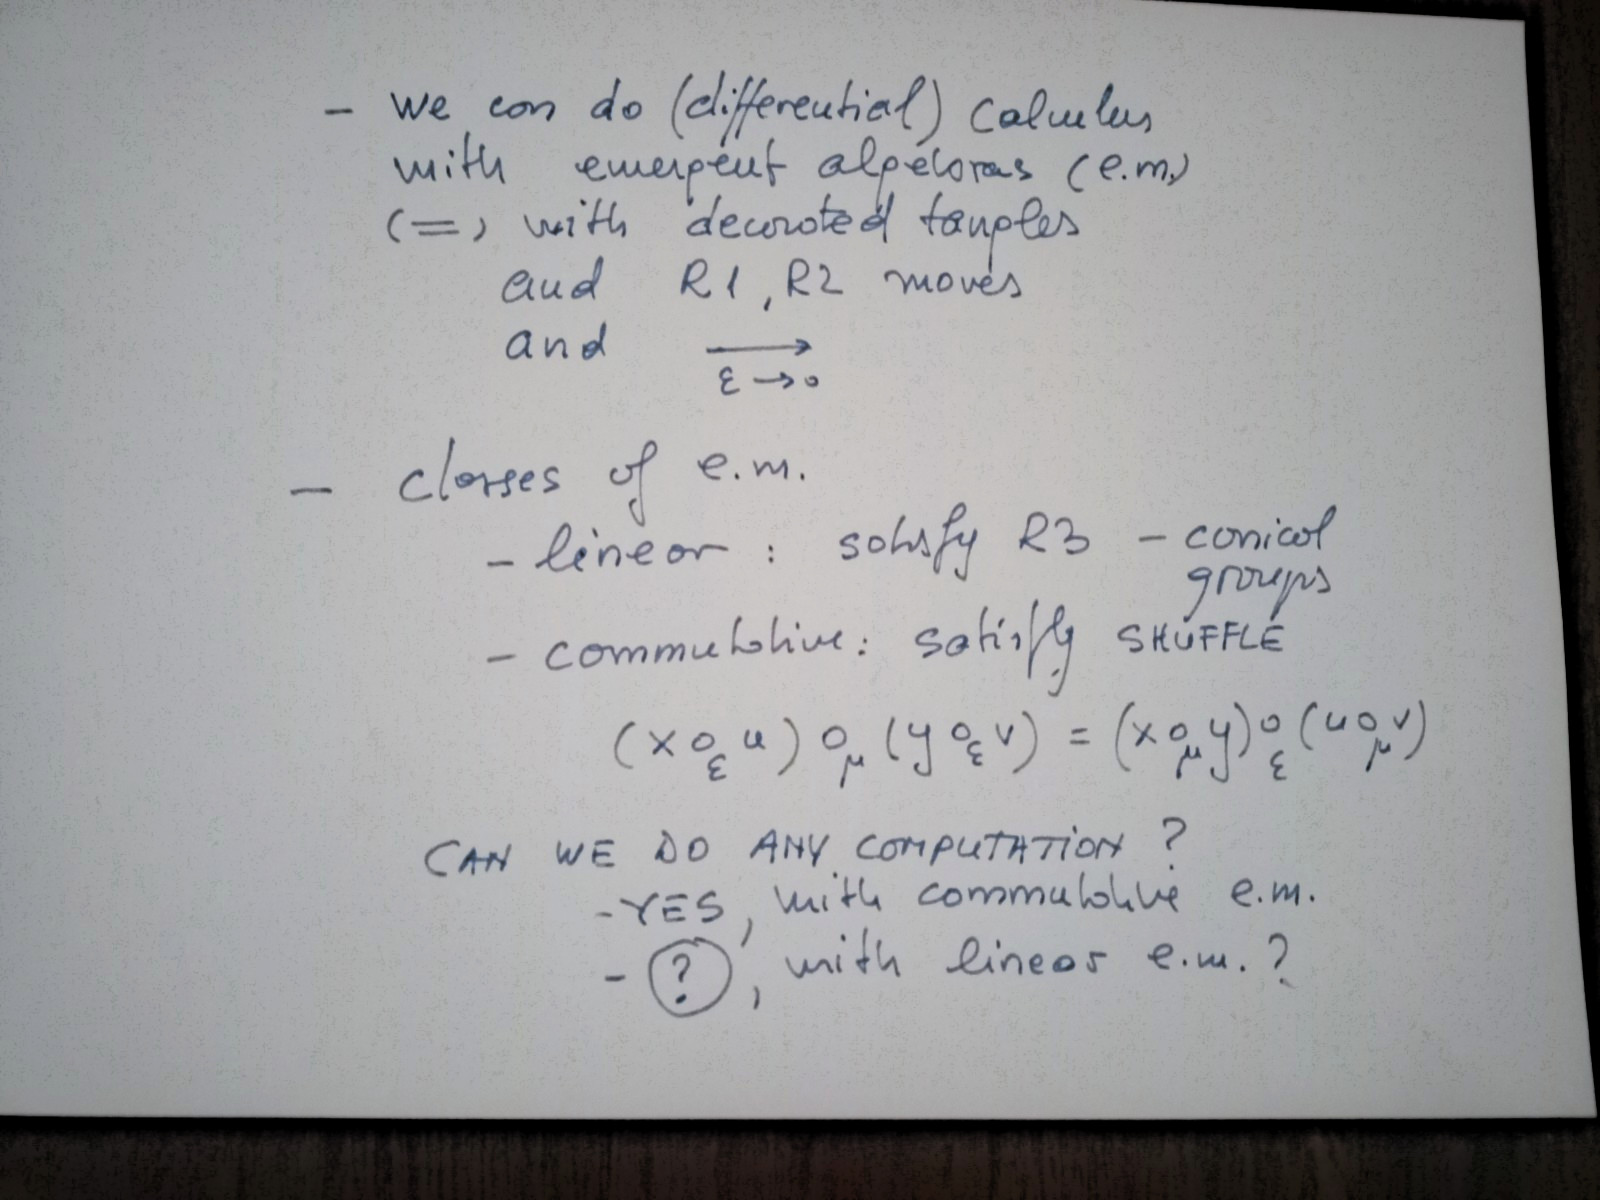
\includegraphics[width=0.75\linewidth]{img/2751.jpg}
\caption{Classes of emergent algebras}
\label{Classes-of-emergent-algebras}
\end{figure}

There are interesting classes of emergent algebras, Figure \ref{Classes-of-emergent-algebras}:

\begin{itemize}
\item
  linear e.a. correspond to calculus on conical groups (Carnot groups
  are a particular class encountered in sub-riemannian geometry, for
  example)
\item
  commutative e.a. which satisfy SHUFFLE (leads to the usual calculus in
  topological vector spaces) In this class you can do any computation
  (\href{https://mbuliga.github.io/quinegraphs/puresee.html}{Pure See})
\end{itemize}

Technically, what I want to know is: can you do universal computation in
the linear case? This corresponds to the initial problem.

\hypertarget{what-means-universal-computation}{%
\subsection{What means universal
computation?}\label{what-means-universal-computation}}

There are many, but among them, 3 ways to define what computation means.
They are equivalent in a precise sense.

Lambda calculus is a term rewrite system.

\begin{figure}[h!]
\centering
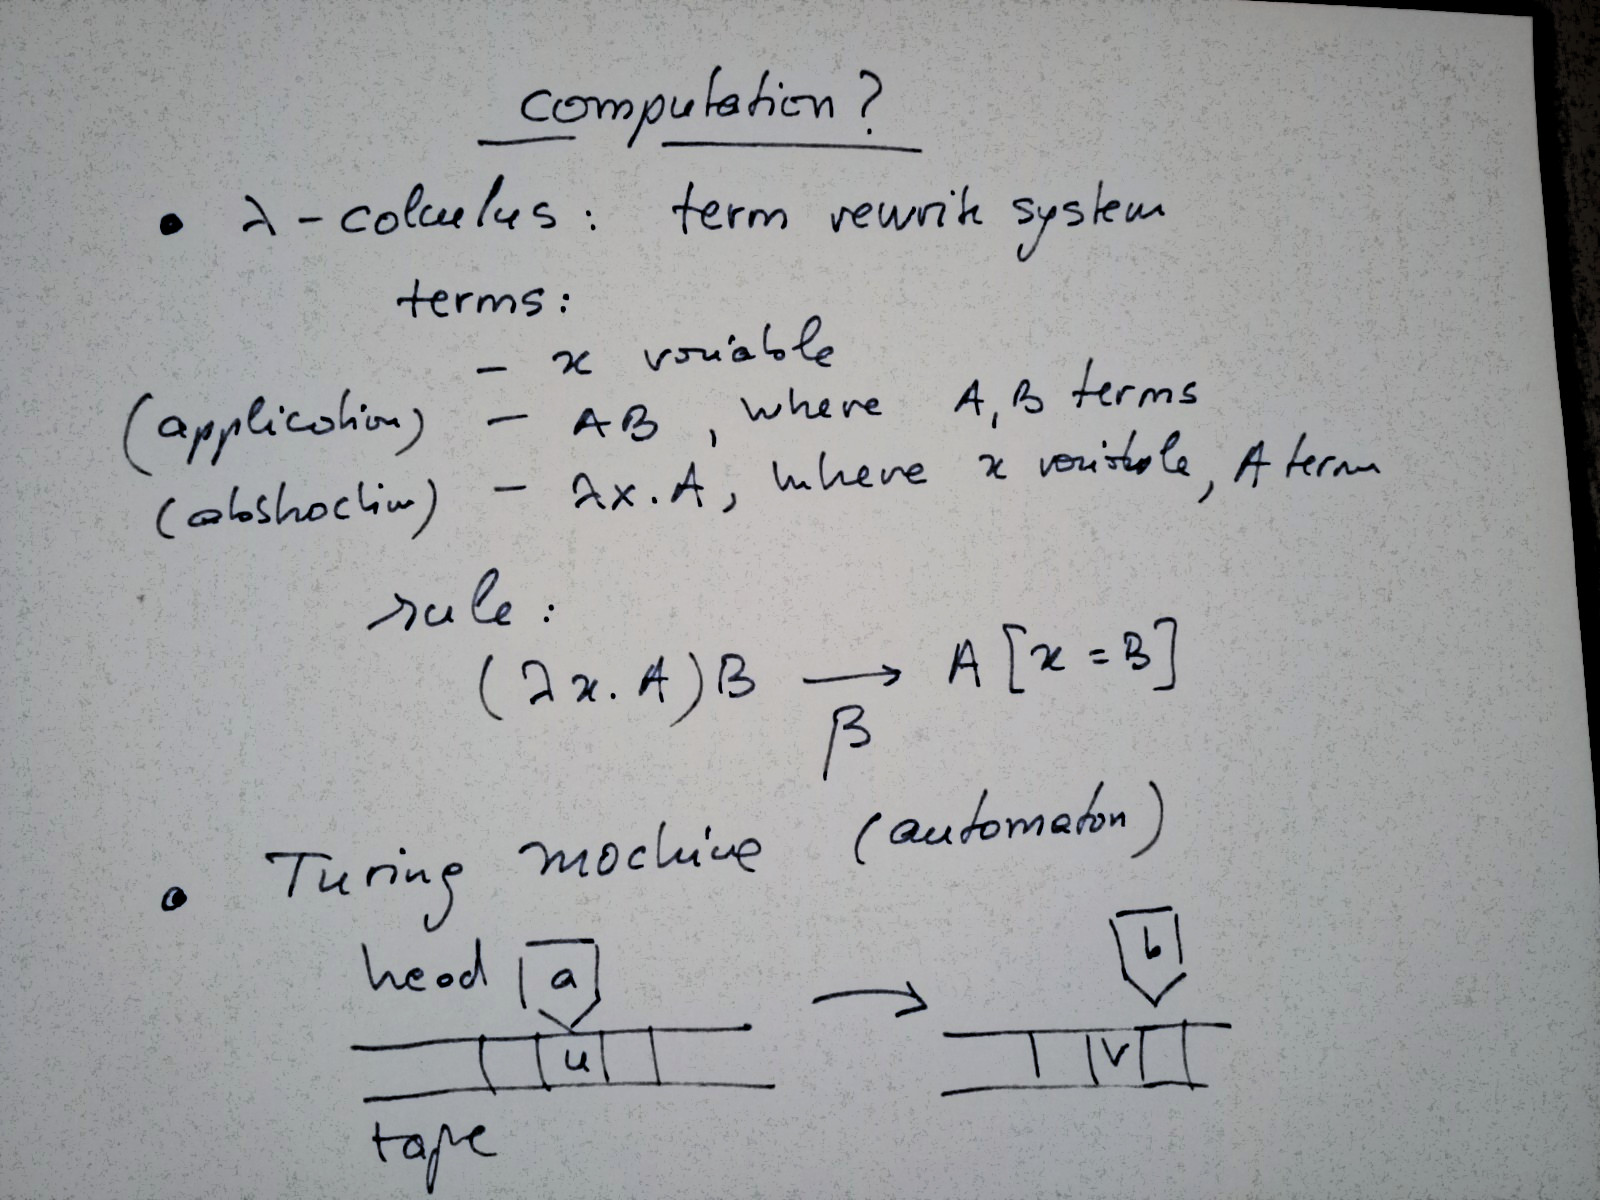
\includegraphics[width=0.75\linewidth]{img/2832.jpg}
\caption{Lambda calculus, Turing machines}
\end{figure}

A Turing machine is an automaton.

Lafont'
\href{https://pdfs.semanticscholar.org/6cfe/09aa6e5da6ce98077b7a048cb1badd78cc76.pdf}{Interaction
Combinators}  \cite{lafont} is a graph rewrite system, where you use graphs with two
types of 3 valent nodes and one type of 1 valent node. Mind that we work
with
\href{http://citeseerx.ist.psu.edu/viewdoc/download?doi=10.1.1.18.5446\&rep=rep1\&type=pdf}{port
graphs} \cite{bawden}, where nodes have numbered ports.

\begin{figure}[h!]
\centering
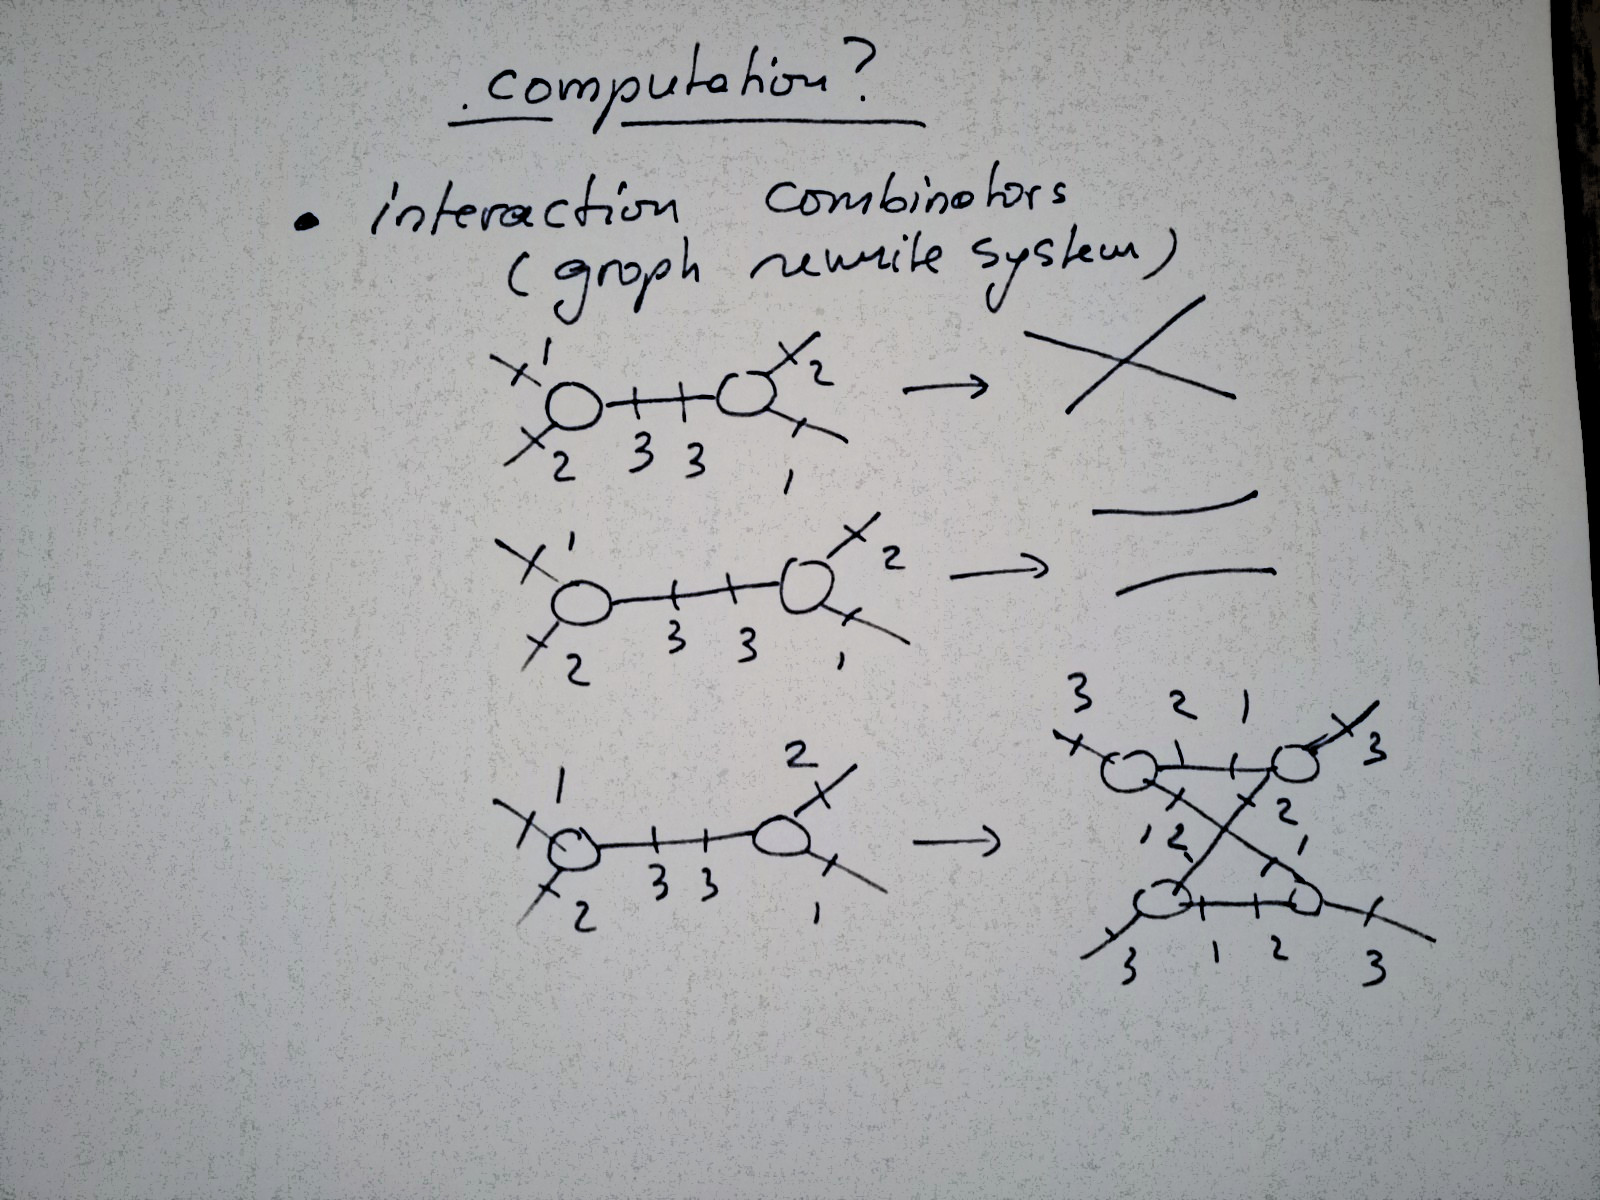
\includegraphics[width=0.75\linewidth]{img/2846.jpg}
\caption{Lafont' Interaction Combinators}
\label{Lafont-Interaction-Combinators}
\end{figure}

Not shown in Figure \ref{Lafont-Interaction-Combinators} are IC rewrites which delete nodes.

Lafont proves that his graph rewrite system is universal because he can
implement Turing machines.

There is a lot of work to implement lambda calculus in a graph rewrite
system, in particular in interaction combinators. The reality is that
this is extremely dificult, in the sense that there are solutions, but
the solutions are not what we want. You can transform a lambda term into
a graph and then reduce it with the graph rewrite system of Lafont, for
example, and then you can decorate the edges of the graph so that you
can retrieve the result of the computation. But while the graph rewrite
system and the algorithm of rewrite applications are local, the parsing
from lambda calculus to graphs and back are non local (there is no a
priori upper bound of the number of nodes and edges involved).
Differently from the graph rewrite systems we are interested in, term
rewrite systems are non-local.
\href{https://telegra.ph/Asemantic-computing-03-02}{See Asemantic
computing}.

We have 3 definition of what computation means, by 3 different models,
which are equivalent only if you add supplementary hypotheses. For me IC
is the most important one, but we don't know yet how to compute with IC
only.

Let me reformulate the problem of if we can compute with R moves.

We can associate a knot quandle to a knot diagram, Figure \ref{Knot-quandle}, simply by naming the
arcs, then we get a presentation of a quandle.

\begin{figure}[h!]
\centering
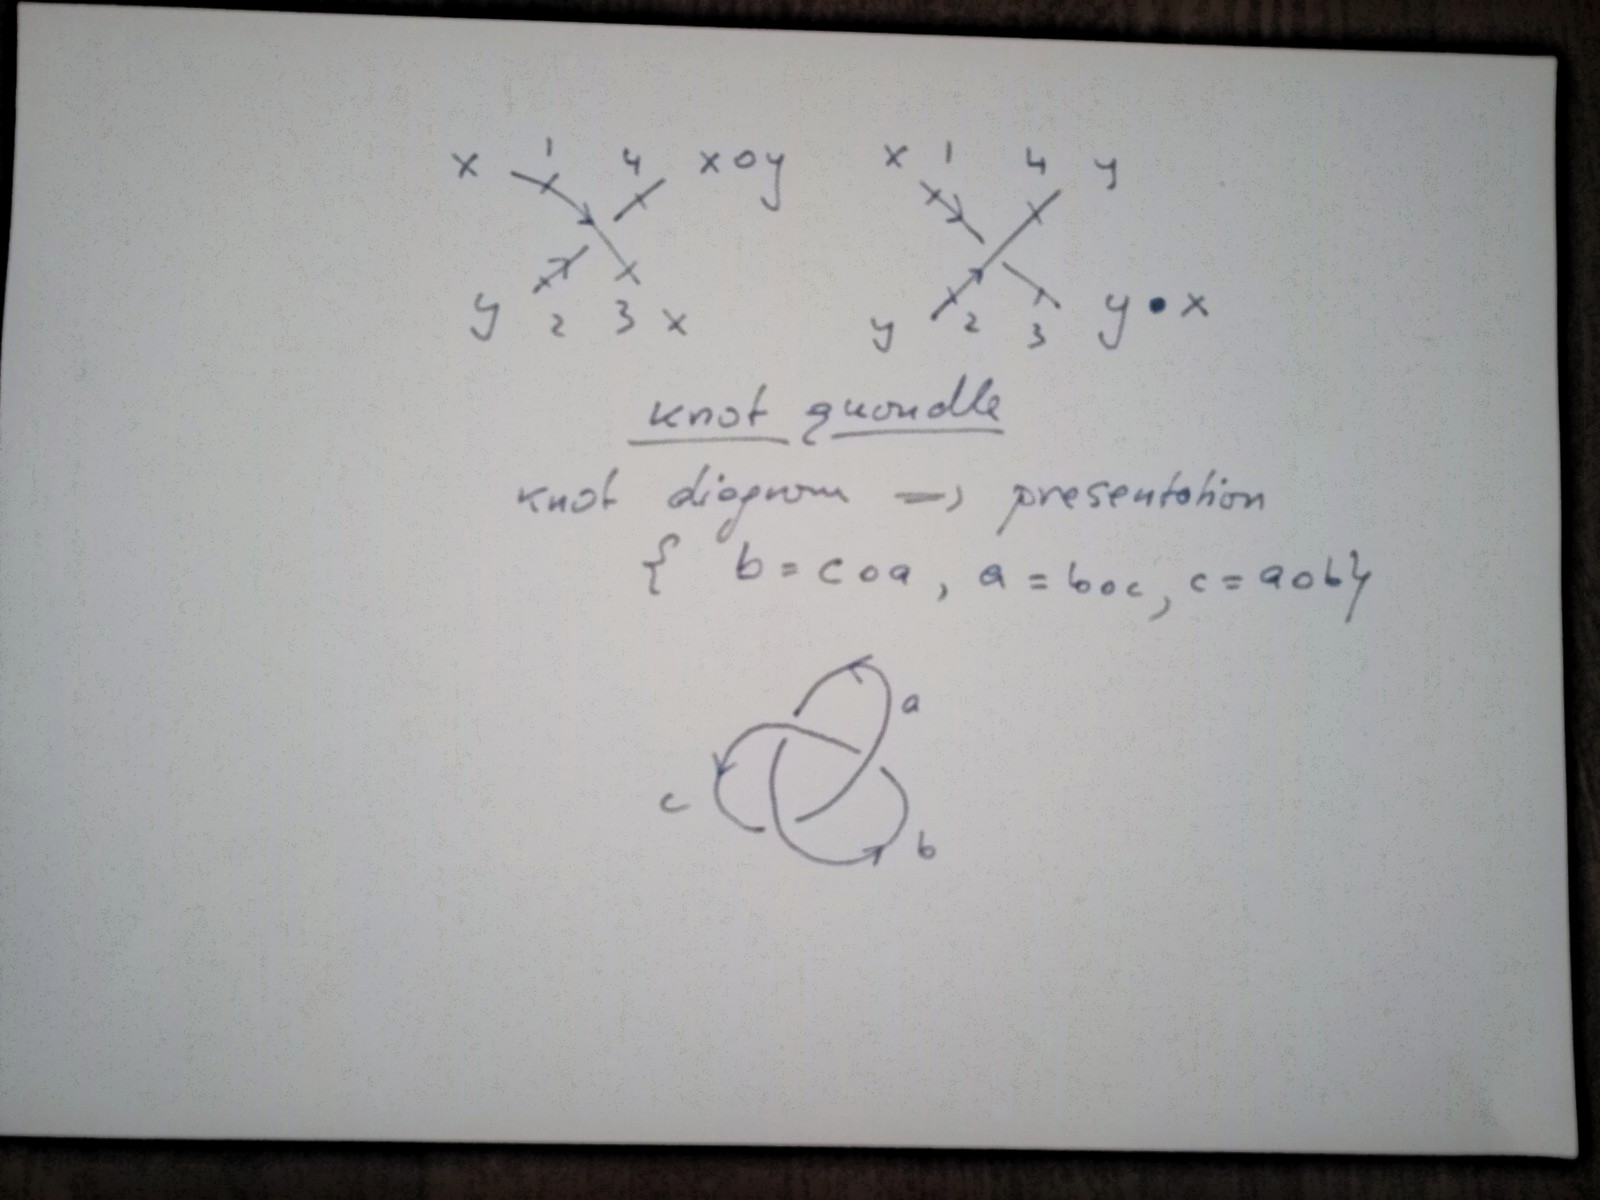
\includegraphics[width=0.75\linewidth]{img/3423.jpg}
\caption{Knot quandle}
\label{Knot-quandle}
\end{figure}

The presentation of a quandle, Figure \ref{Quandle-presentation-in-mol-notation-I} and Figure \ref{Quandle-presentation-in-mol-notation-II} is invariant with respect to the
permutation of relations or the renaming of the arcs. There is a small
problem, we have to introduce fanin and fanout nodes too. For example
when an arc passes over two crossings, we have a hidden fanout. The
solution is to use a different notation and FIN (fanin) and FO (fanout)
nodes. This turns the presentation into a
\href{https://arxiv.org/abs/2003.14332}{mol file} \cite{buligageneral}, like described in the
following figure.

\begin{figure}[h!]
\centering
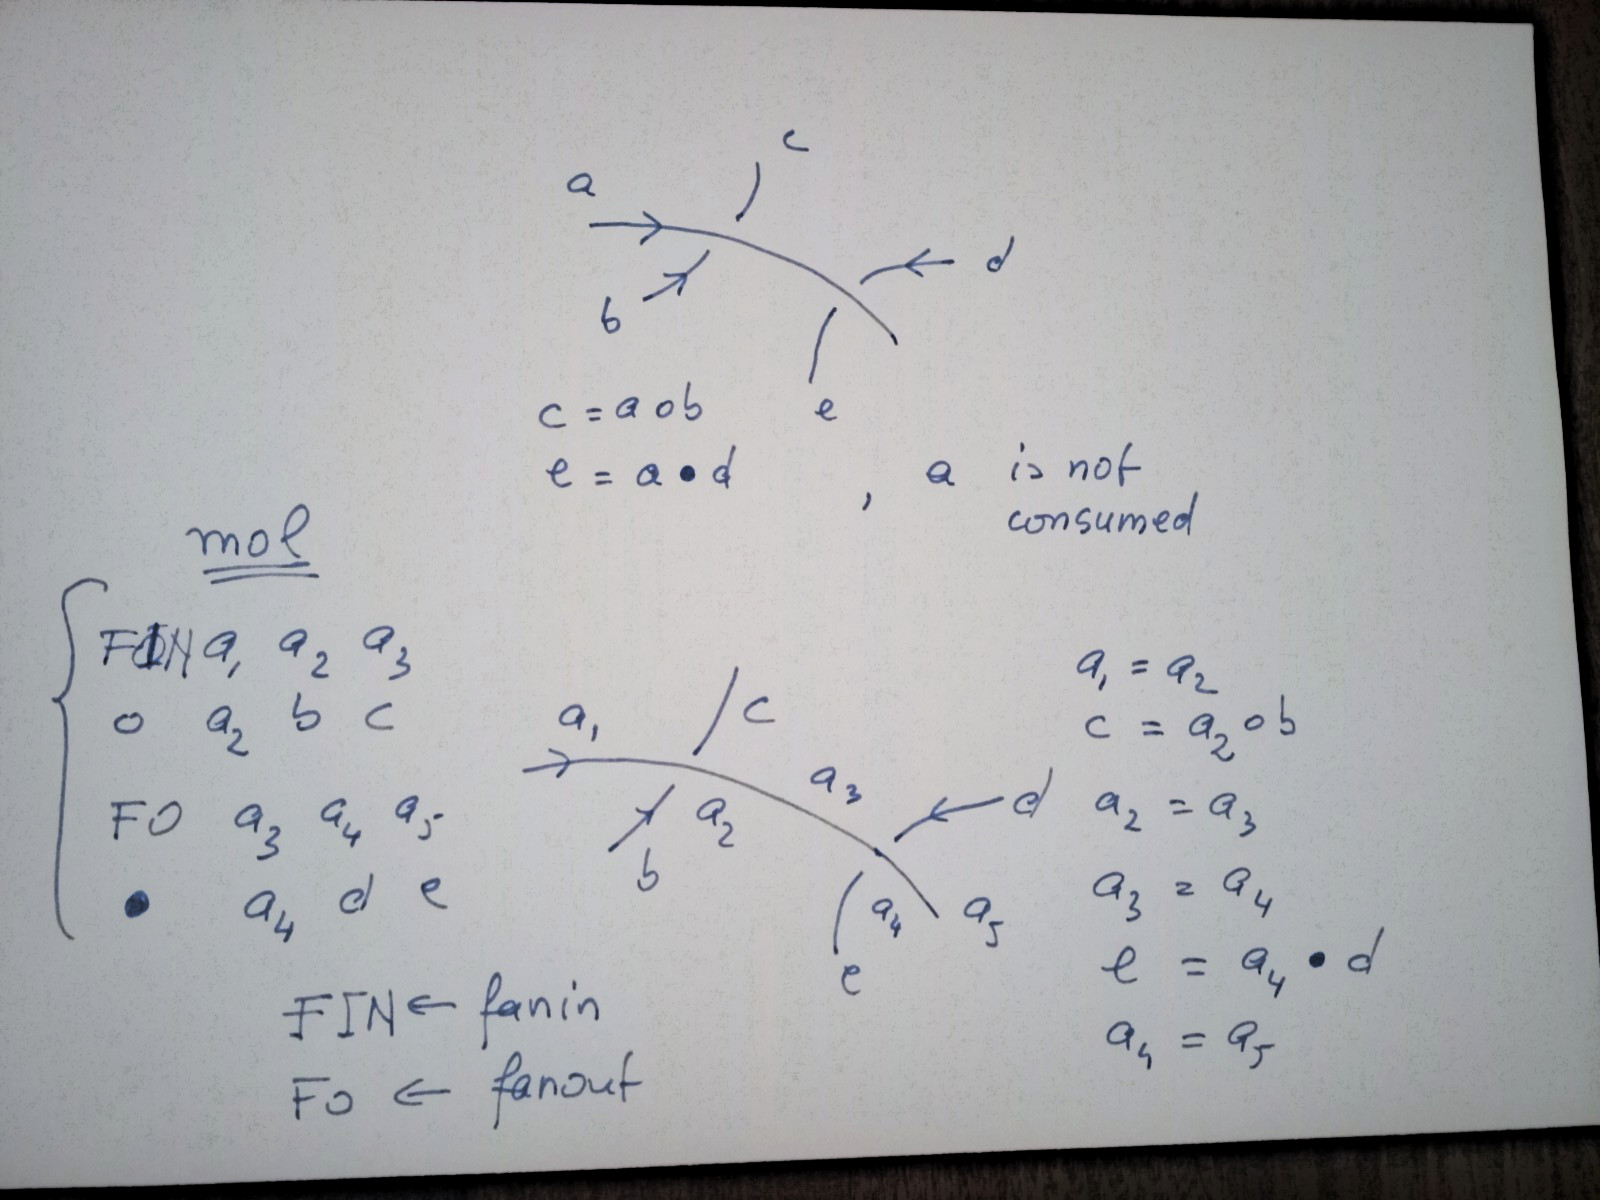
\includegraphics[width=0.75\linewidth]{img/3439.jpg}
\caption{Quandle presentation in mol notation I}
\label{Quandle-presentation-in-mol-notation-I}
\end{figure}

\begin{figure}[h!]
\centering
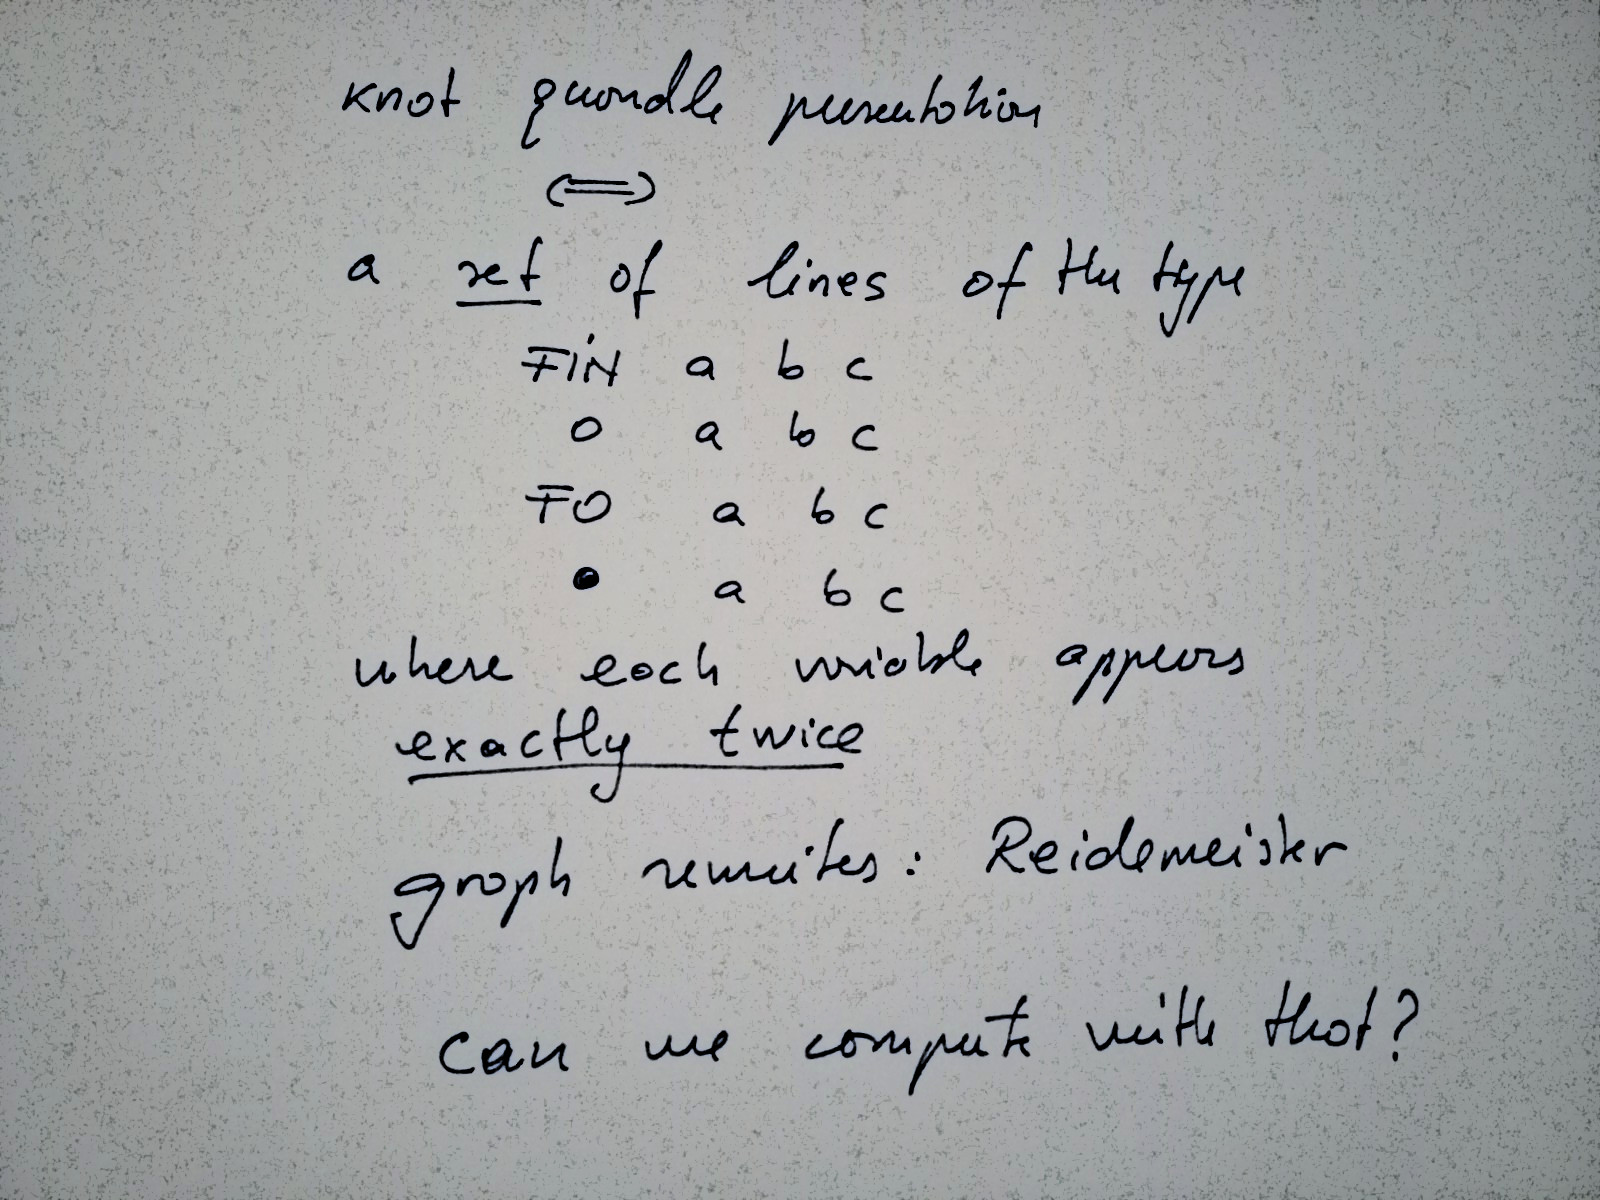
\includegraphics[width=0.75\linewidth]{img/3450.jpg}
\caption{Quandle presentation in mol notation II}
\label{Quandle-presentation-in-mol-notation-II}
\end{figure}

Can we compute with that?

\textbf{Theorem.} If there is a parser from lambda calculus to knot
diagrams, such that any lambda calculus rewrite is parsed to a pair of
knot diagrams which are equivalent under the Reidemeister moves, and
such that there is a term sent to a diagram of the unknot, then all
lambda terms are sent to diagrams of the unknot.

The proof is simple. Let A be the non empty set of all lambda terms
which are parsed to a diagram of an unknot and let B the set of all
other lambda terms. By Haken we have an algorithm to detect the unknot
and the Scott-Curry theorem tells us that B has to be empty.

This shows that we can't hope to do computations with tangle diagrams
and R moves only, with the algorithm of random application of rewrites
(or with any local algorithm), because if we could then we can also turn
any graph representing a lambda term to the unknot.

We can compute with knot diagrams, but in a stupid way: if we use
diagrams as a notational device.

\begin{figure}[h!]
\centering
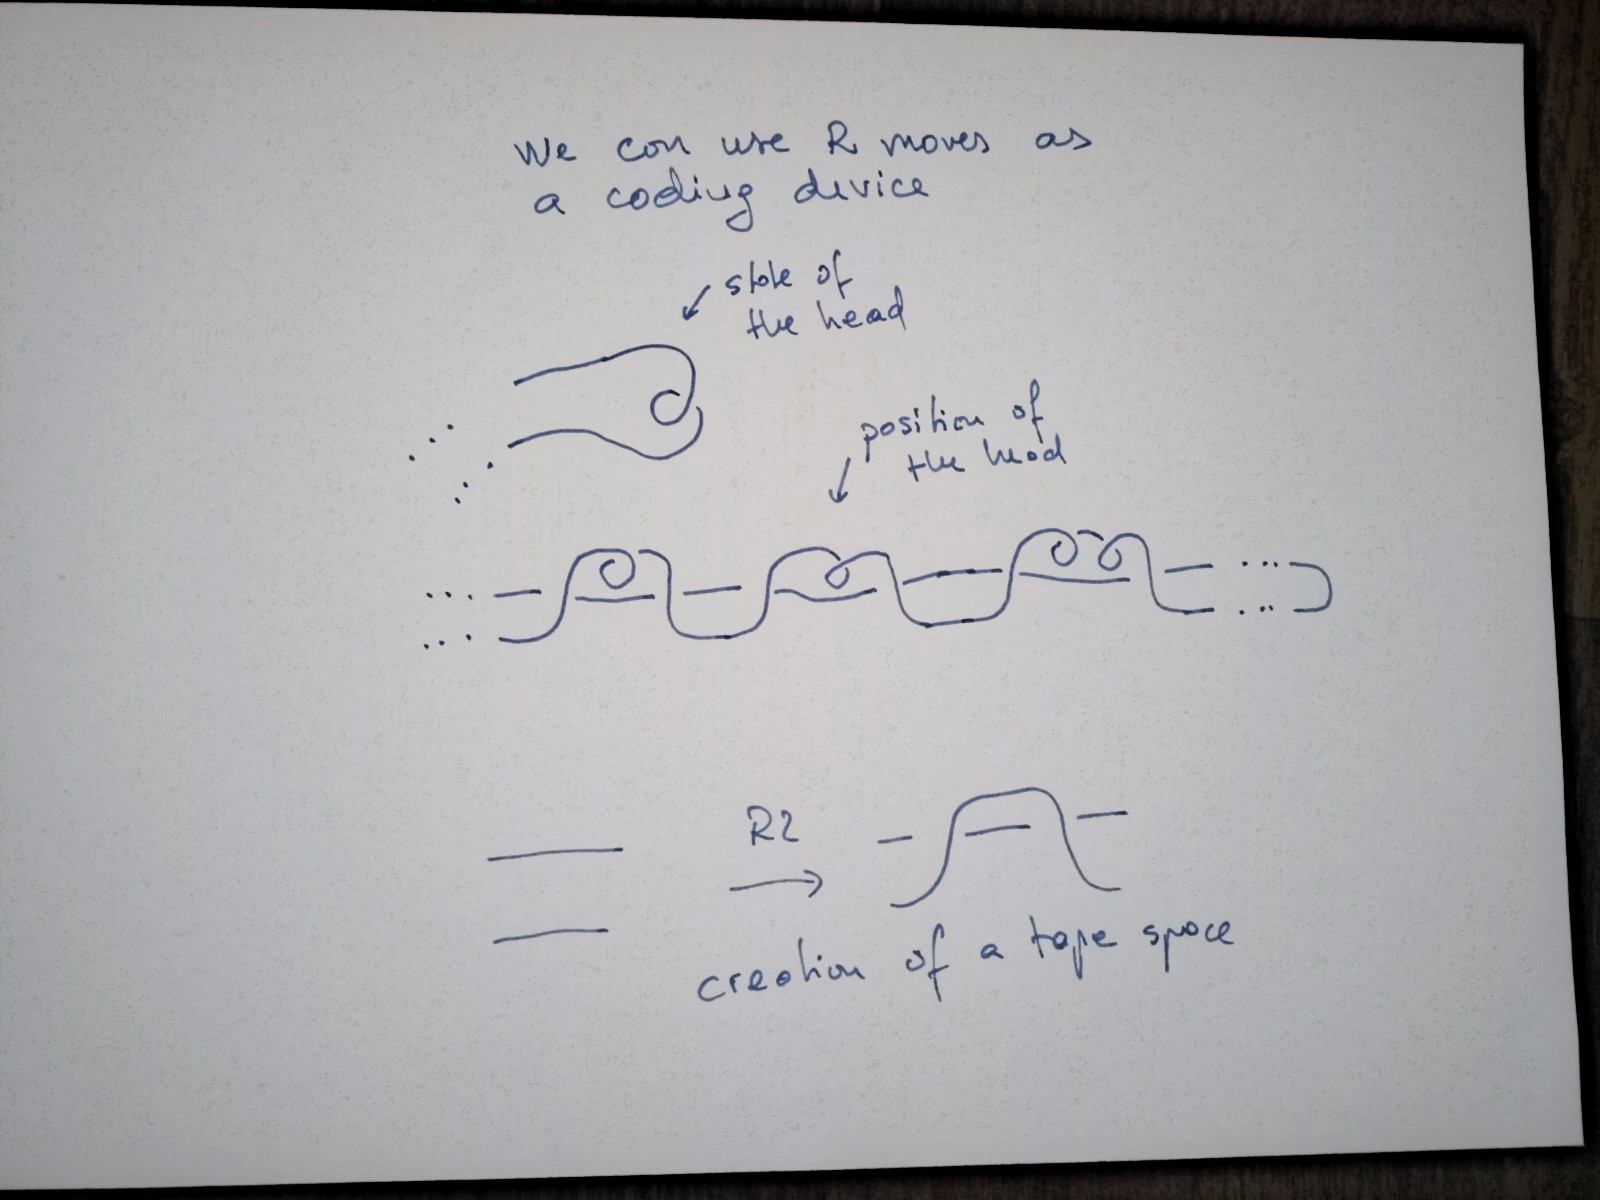
\includegraphics[width=0.75\linewidth]{img/3633.jpg}
\caption{Turing machine with tangles and R moves}
\label{Turing-machine-with-tangles-and-R-moves}
\end{figure}

Indeed, as described in Figure \ref{Turing-machine-with-tangles-and-R-moves},take an unknot, flatten it and use parts of it for the head state and other parts for the tape symbols. The computation is then
realized via R moves, but there are sequences or R moves which turn the
diagram into the unknot, which do not correspond to a Turing machine
computation. You may add variations where we use such diagrams for
headless Turing machines, or even for another universal computation
model, the SKI combinators calculus
\href{https://mbuliga.github.io/chemski/chemski.html\#SKInote}{via
chemSKI}. We can't hope to use only the R moves, in a local way, to do 
universal computation.

\hypertarget{zip-slip-smash}{%
\subsection{Zip-Slip-Smash}\label{zip-slip-smash}}

I argue that we need to introduce a way to reconnect edges. For this I
introduce zippers. The idea is that a zipper is a thing which has two
non-identical parts, so it's made of two half-zippers, which are not
identical. There will be two types of zippers: black and white. We also
have ends (black and white) which are 1 valent, and of course crossings
of two types, which are 4 valent nodes. In Figure \ref{The-elements-of-ZSS} we see the elements of ZSS.

\begin{figure}[h!]
\centering
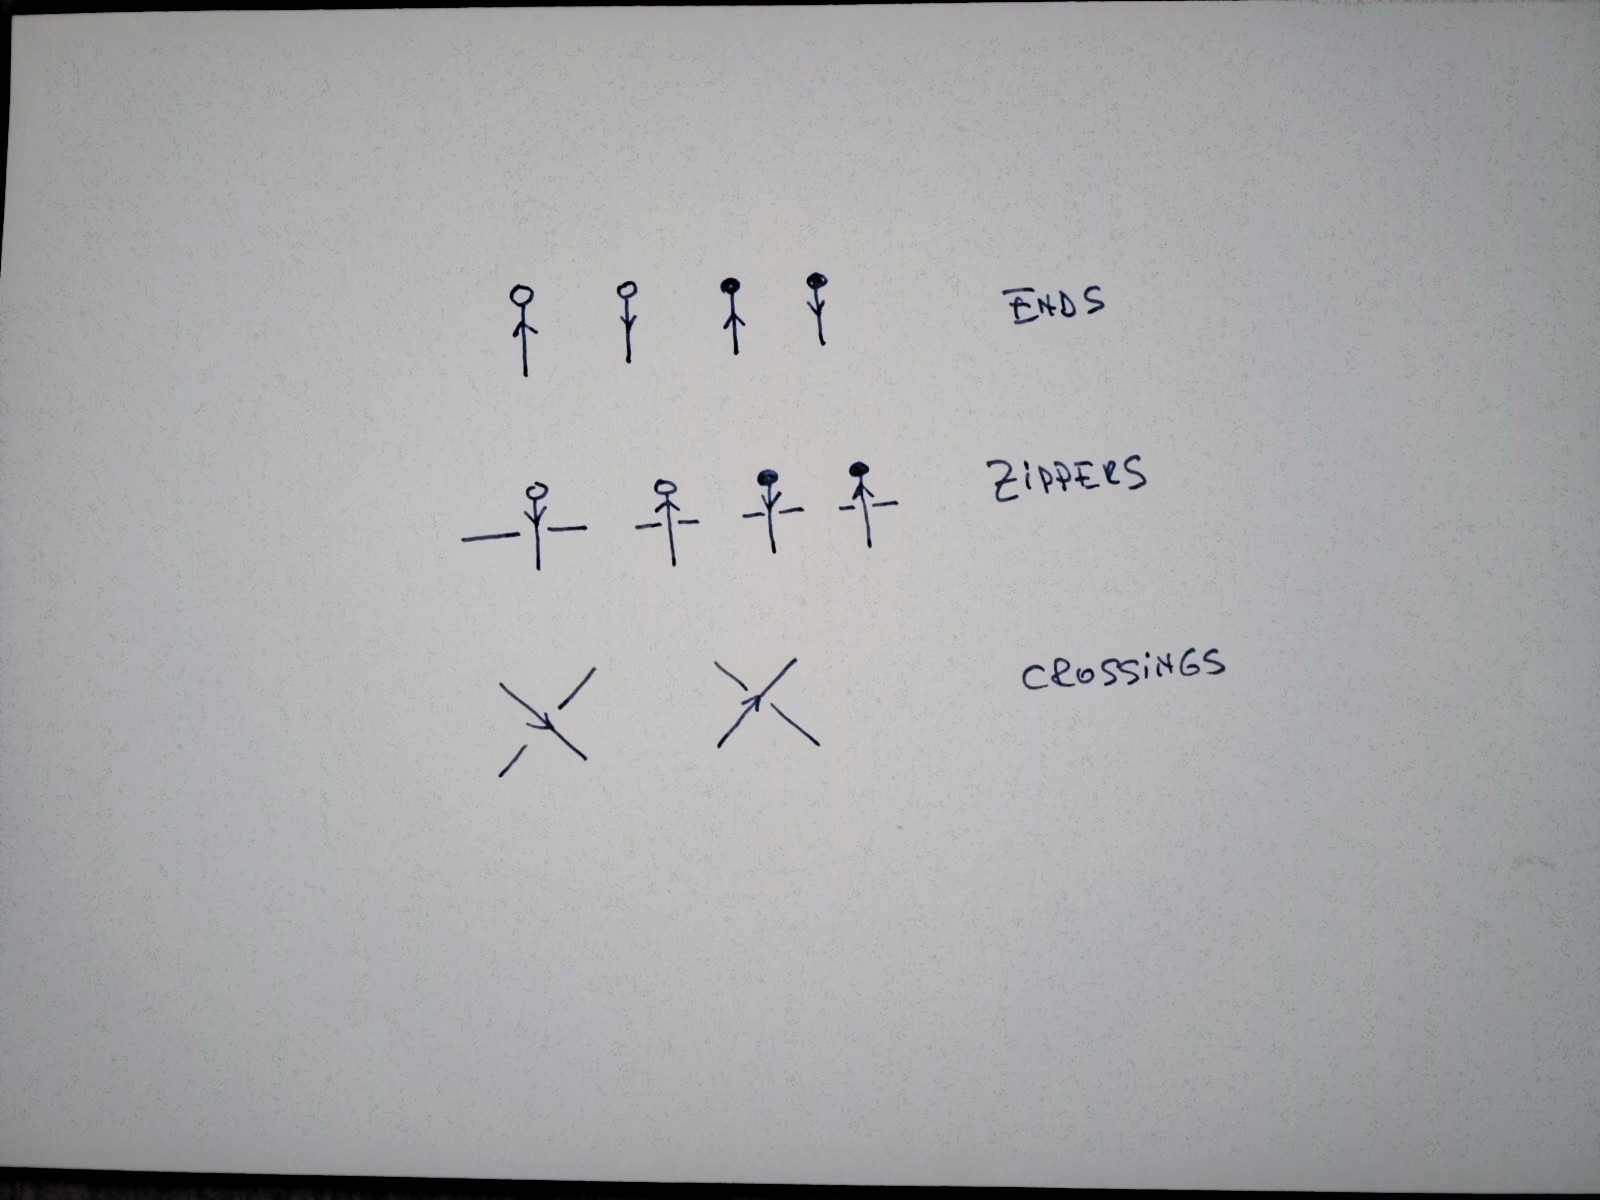
\includegraphics[width=0.75\linewidth]{img/3647.jpg}
\caption{The elements of ZSS}
\label{The-elements-of-ZSS}
\end{figure}

There are 4 types of half-zippers (two white, two black). In Figure \ref{4-types-of-half-zippers} you see
them also in the mol notation.

\begin{figure}[h!]
\centering
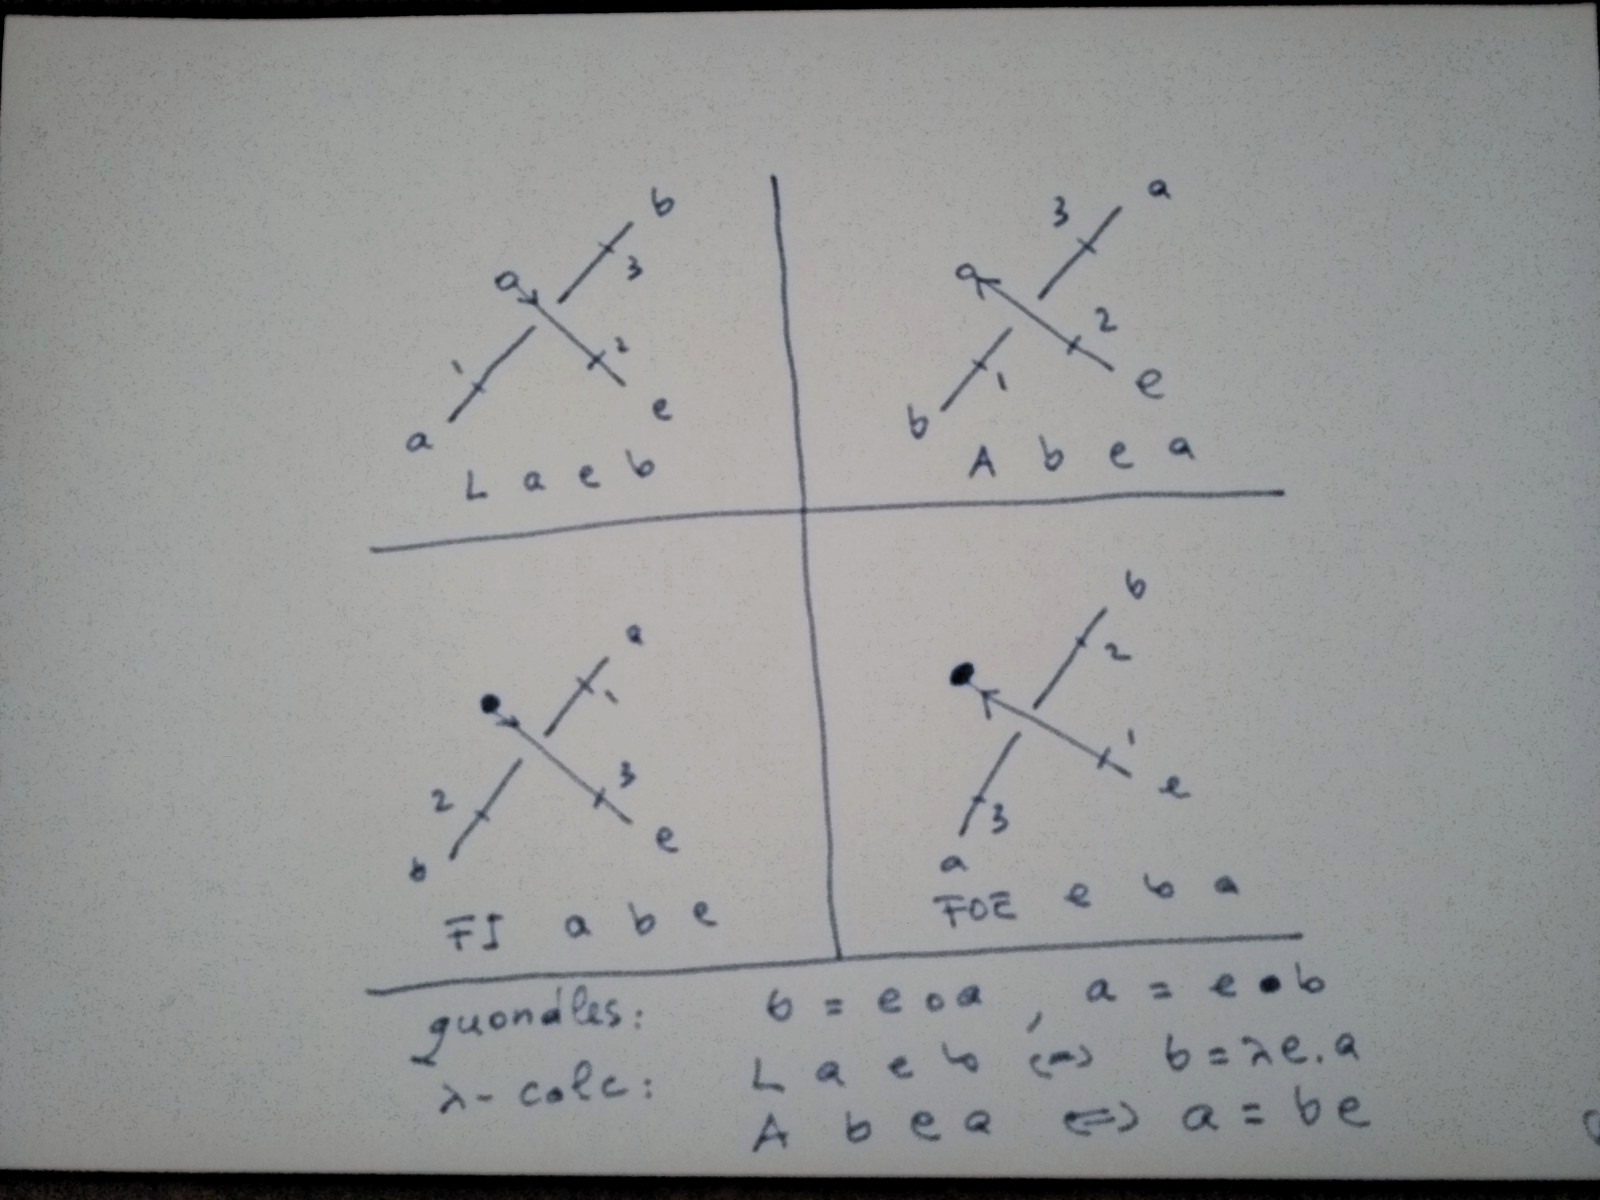
\includegraphics[width=0.75\linewidth]{img/3704.jpg}
\caption{4 types of half-zippers}
\label{4-types-of-half-zippers}
\end{figure}

The L and A half-zippers are related to the lambda calculus abstraction
and application operations, like in \cite{chemlambda} 
\href{https://mbuliga.github.io/quinegraphs/history-of-chemlambda.html\#ChemlambdaV2}{chemlambda}.

We also have crossings, which are 4 valent nodes, Figure \ref{2-types-of-crossings}. Each crossing is
represented in the mol notation by a pair of lines.

\begin{figure}[h!]
\centering
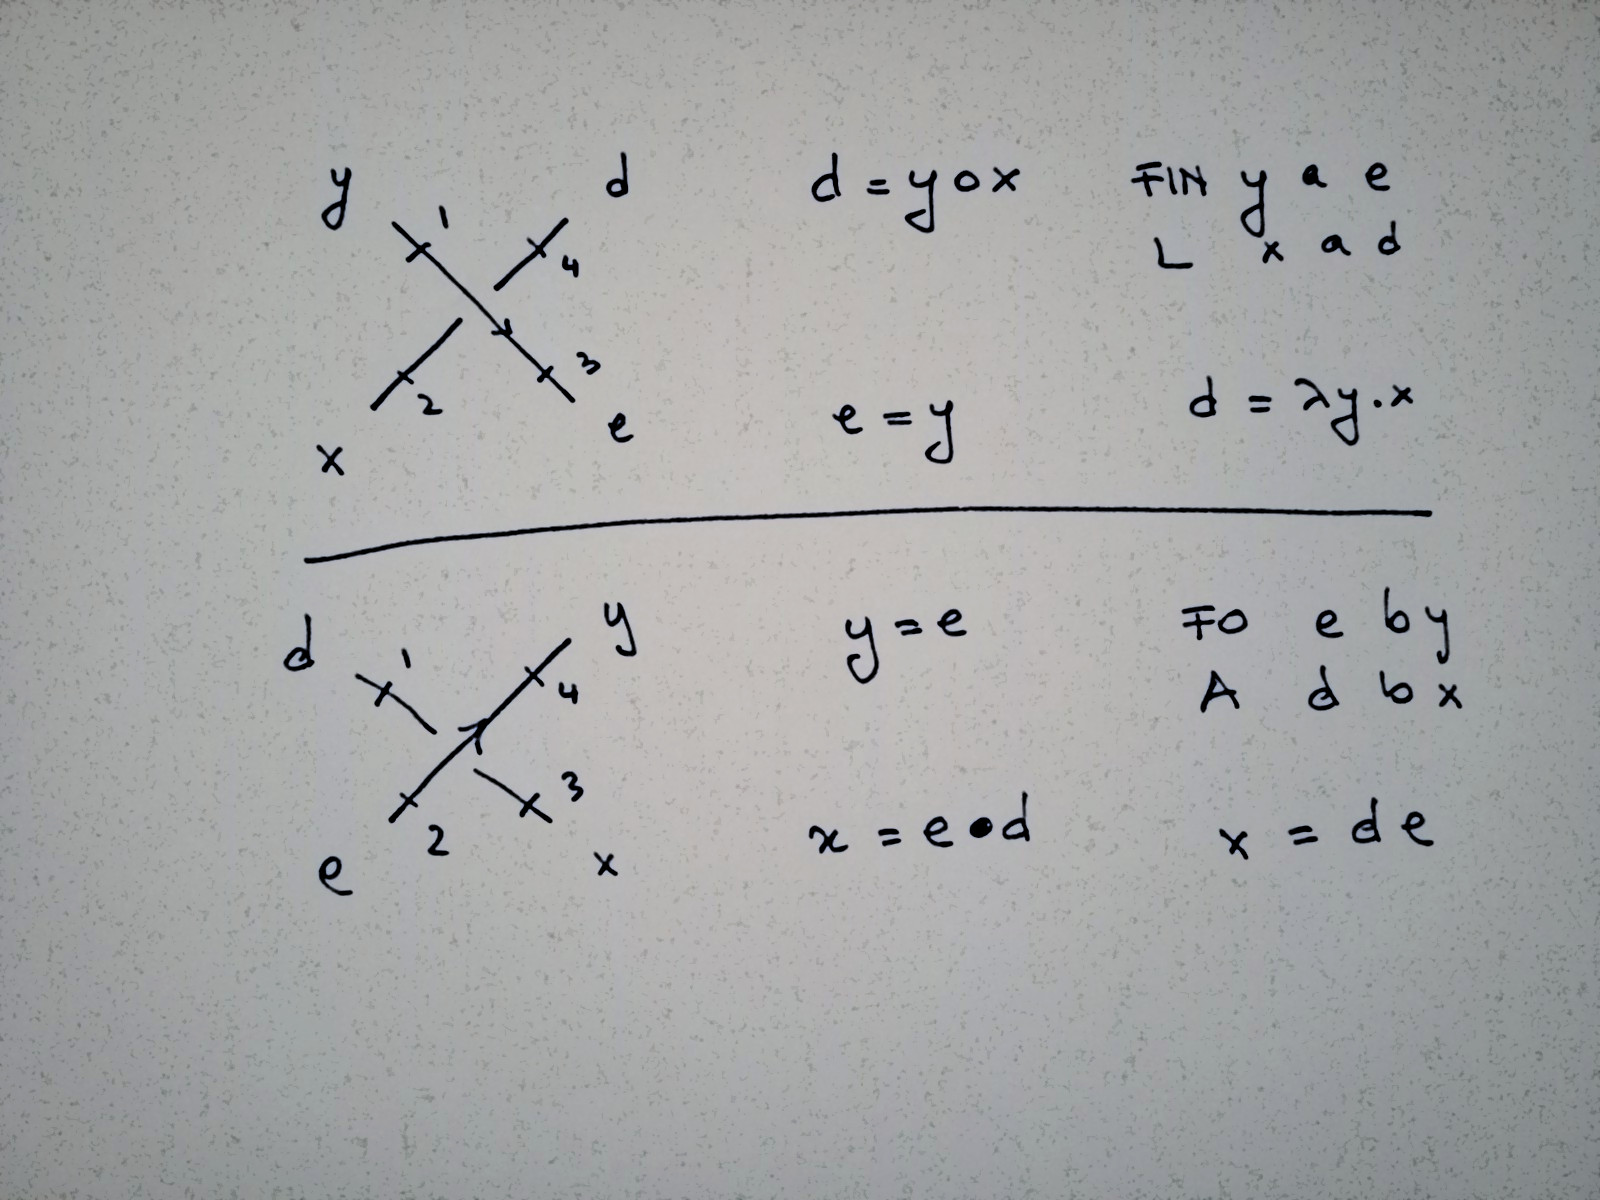
\includegraphics[width=0.75\linewidth]{img/3716.jpg}
\caption{2 types of crossings}
\label{2-types-of-crossings}
\end{figure}

This corresponds to the usual way to see a crossing (which is 4 valent)
as if it is a pair of two 3 valent nodes, one of them being a fanin
(FIN) or a fanout (FO).

Now let's see the rewrites which give the name of ZSS: zip, slip, smash.

There are two \textbf{zip rewrites}. The first one, Figure \ref{First-zip-rewrite}, uses only white
half-zippers.

\begin{figure}[h!]
\centering
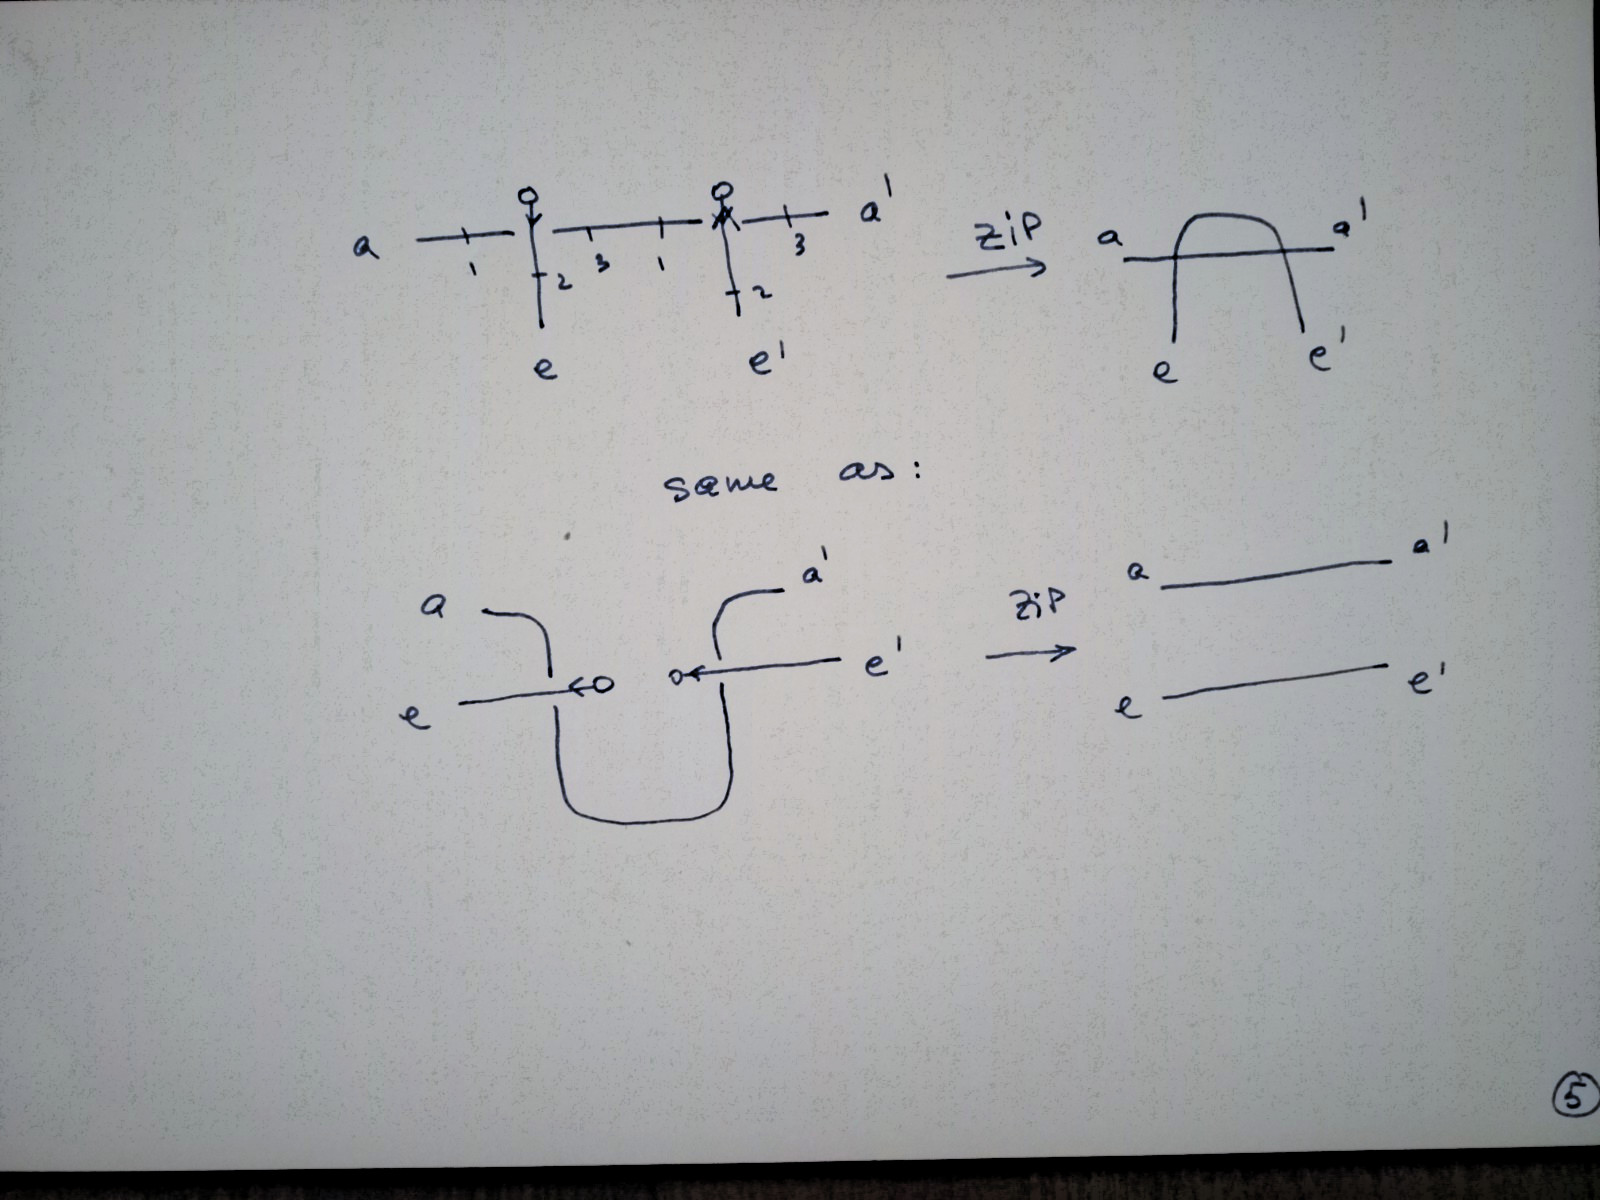
\includegraphics[width=0.75\linewidth]{img/3748.jpg}
\caption{First zip rewrite}
\label{First-zip-rewrite}
\end{figure}

It can be used to make diagrams and rewrites which really look like
zippers, Figure \ref{White-zipper}.

\begin{figure}[h!]
\centering
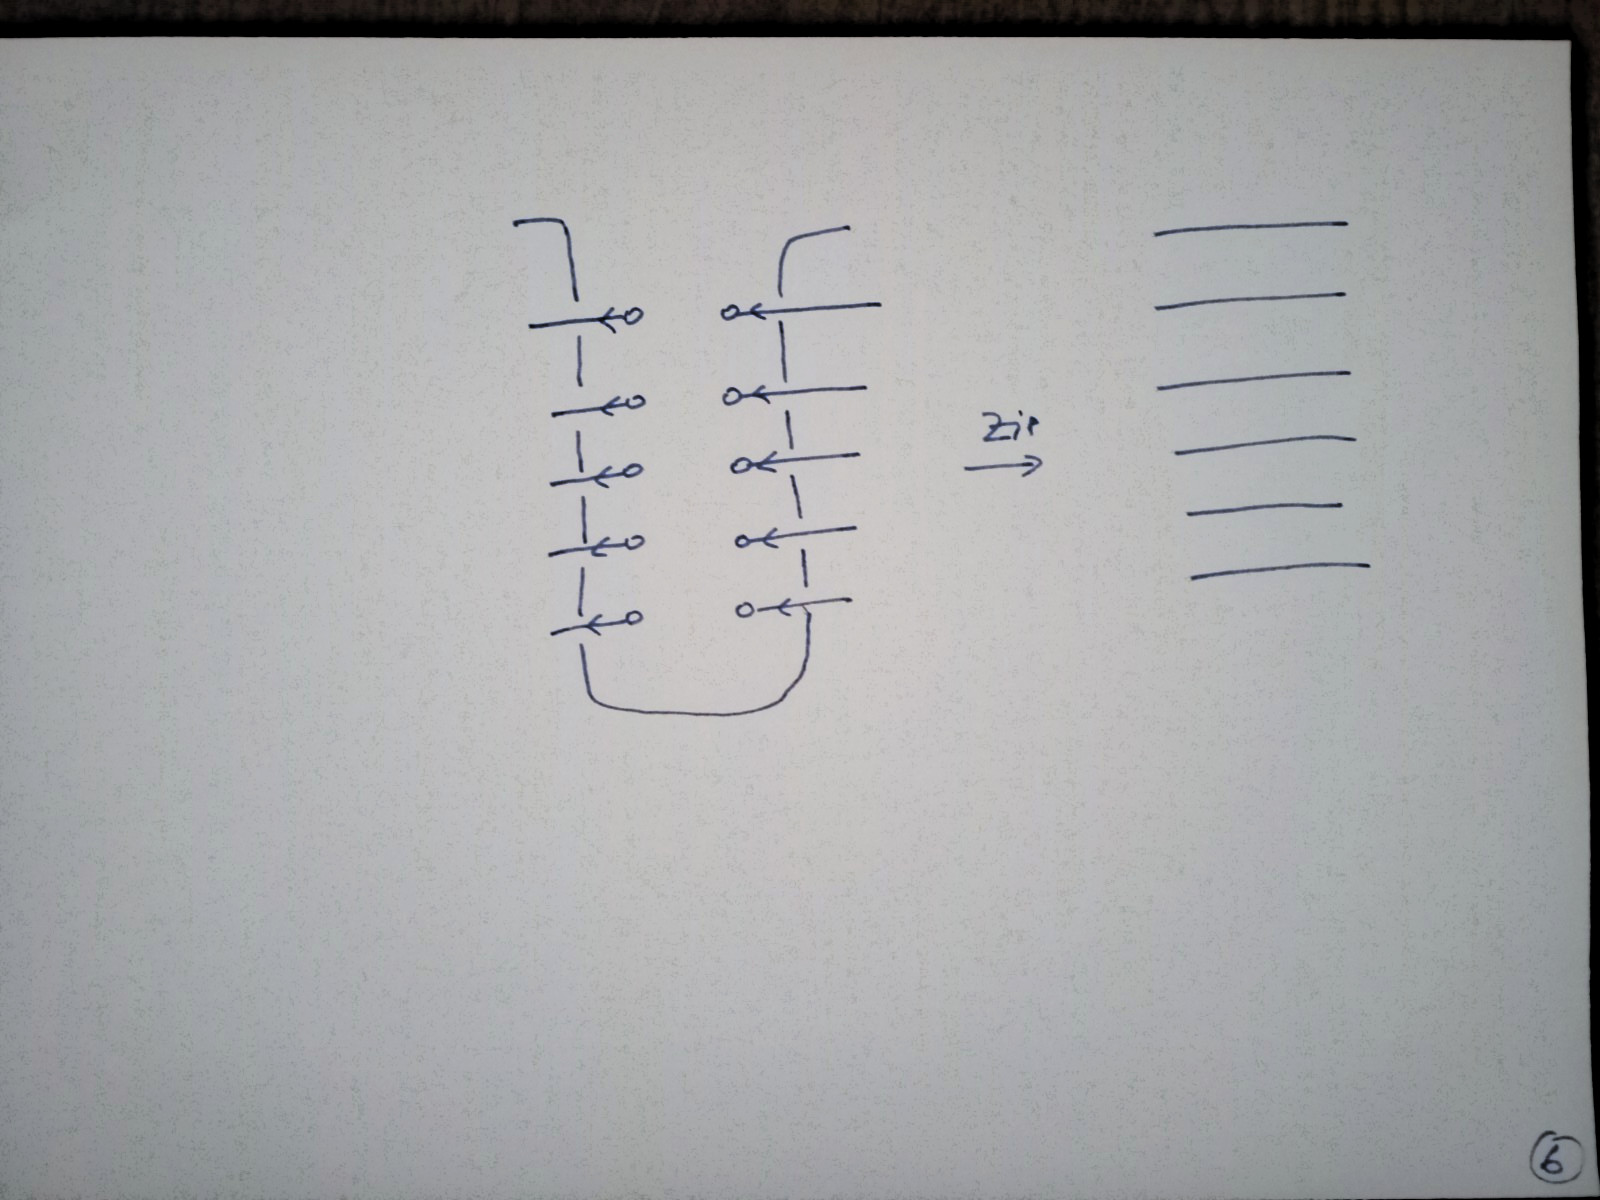
\includegraphics[width=0.75\linewidth]{img/3807.jpg}
\caption{White zipper}
\label{White-zipper}
\end{figure}

The second zip rewrite, Figure \ref{Second-zip-rewrite-and-black-zippers}, uses only black half-zippers:

\begin{figure}[h!]
\centering
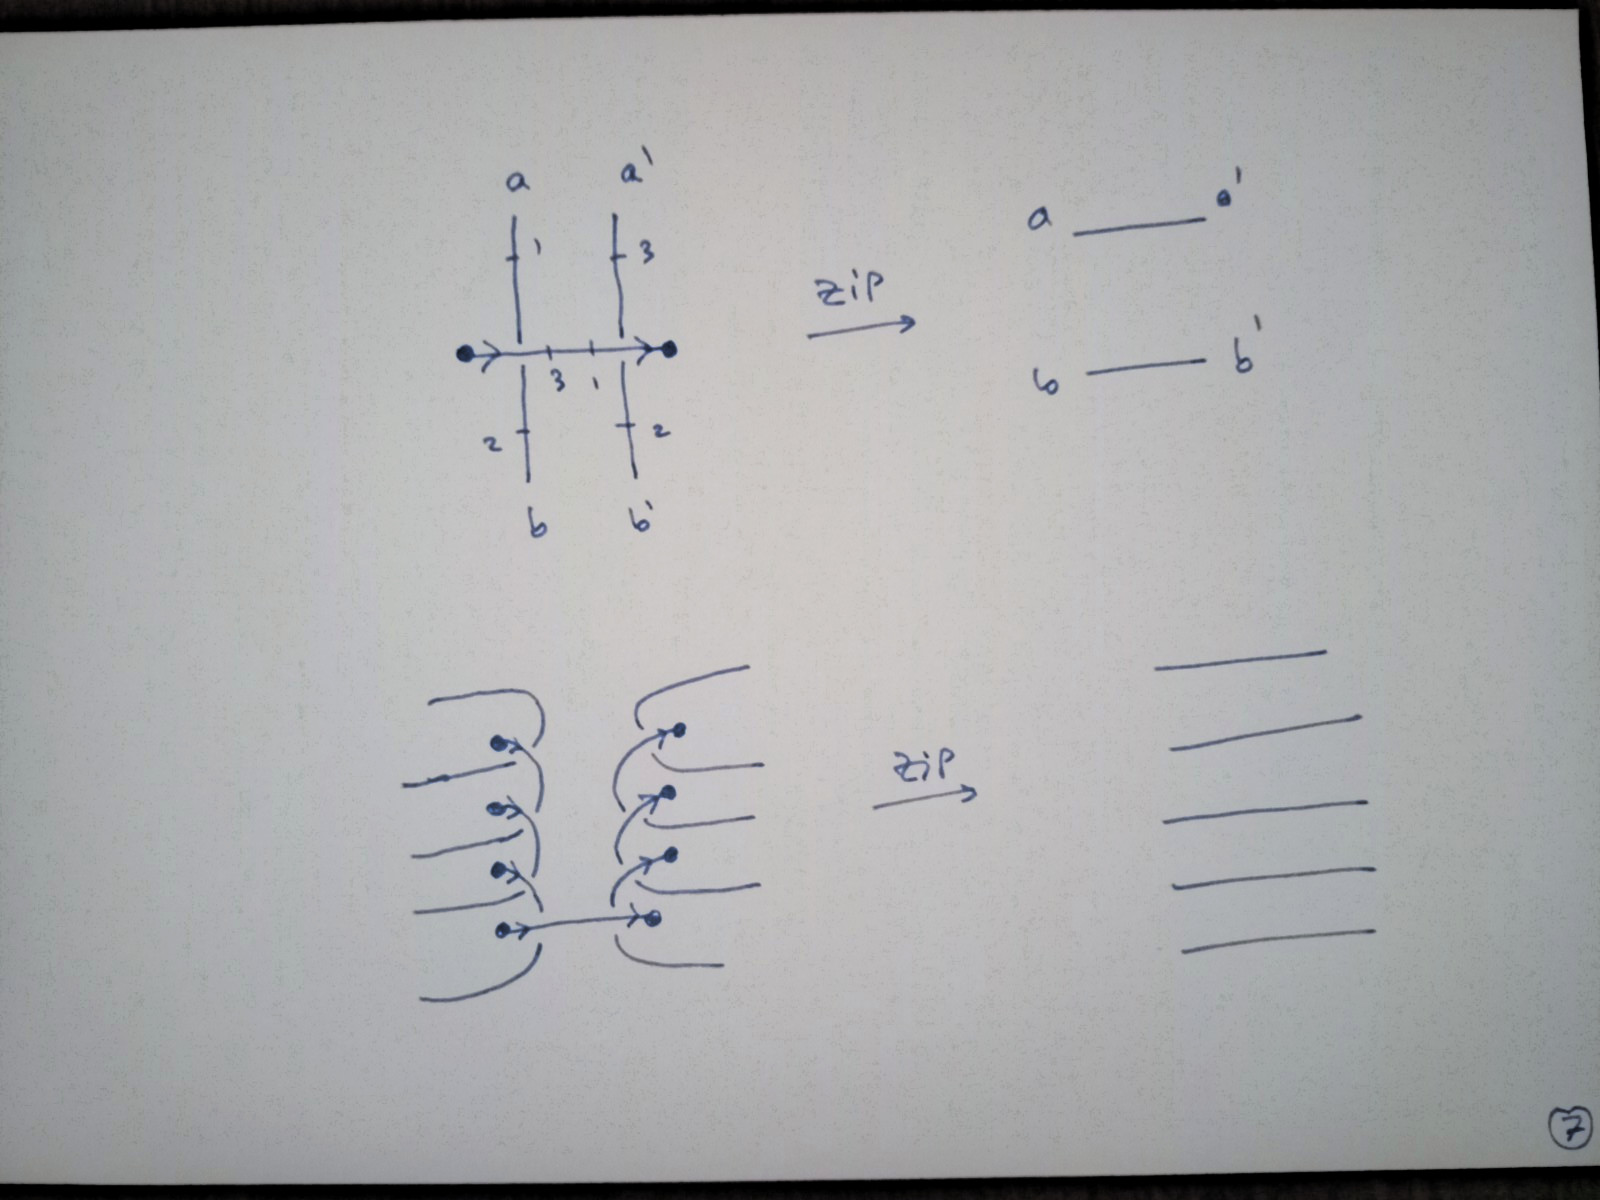
\includegraphics[width=0.75\linewidth]{img/3821.jpg}
\caption{Second zip rewrite and black zippers}
\label{Second-zip-rewrite-and-black-zippers}
\end{figure}

With this we can make black zippers as well.

The \textbf{slip rewrites} are introduced, Figure  \ref{The-slip-rewrites}, because there is a graphical
ambiguity in the drawing of a half-zipper. We see there an end (black or
white) and a crossing, or is there a black or white half-zipper?

\begin{figure}[h!]
\centering
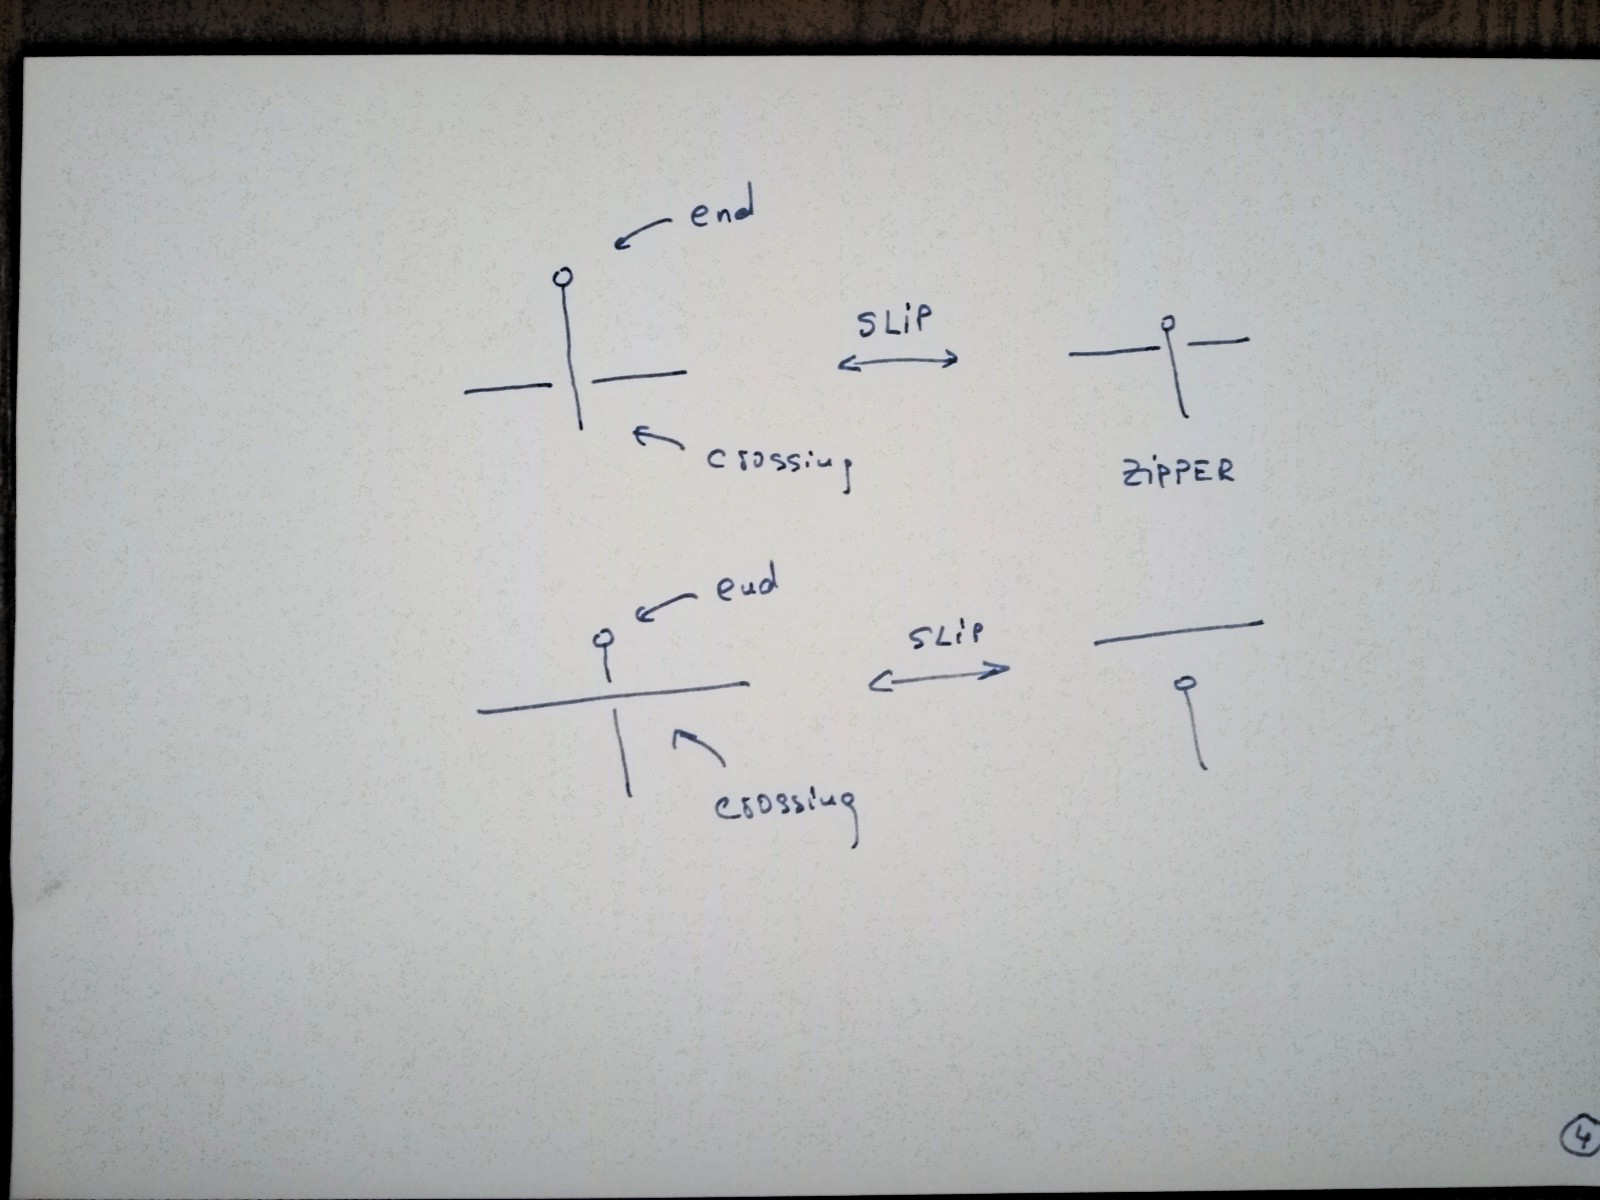
\includegraphics[width=0.75\linewidth]{img/3731.jpg}
\caption{The slip rewrites}
\label{The-slip-rewrites}
\end{figure}

The slip rewrites tell us that ends (of any color) which pass over the
crossing are the same as half-zippers, and also that ends which pass
under the crossing \ldots{} slip under and the crossing is destroyed. S.
Carter mentions that such rewrites appear also in \cite{carter} Geometric
Interpretations of Quandle Homology
\href{https://arxiv.org/abs/math/0006115v1}{arXiv:math/0006115v1} .

The \textbf{smash rewrites} create half-zippers. Imagine that you smash
a crossing with a hammer and it breaks down into two half-zippers. (Mind
that all rewrites are bi-directional though, so you can also turn a pair
of half-zippers into a crossing). The first smash rewrite is in Figure \ref{The-first-smash-rewrite}.

\begin{figure}[h!]
\centering
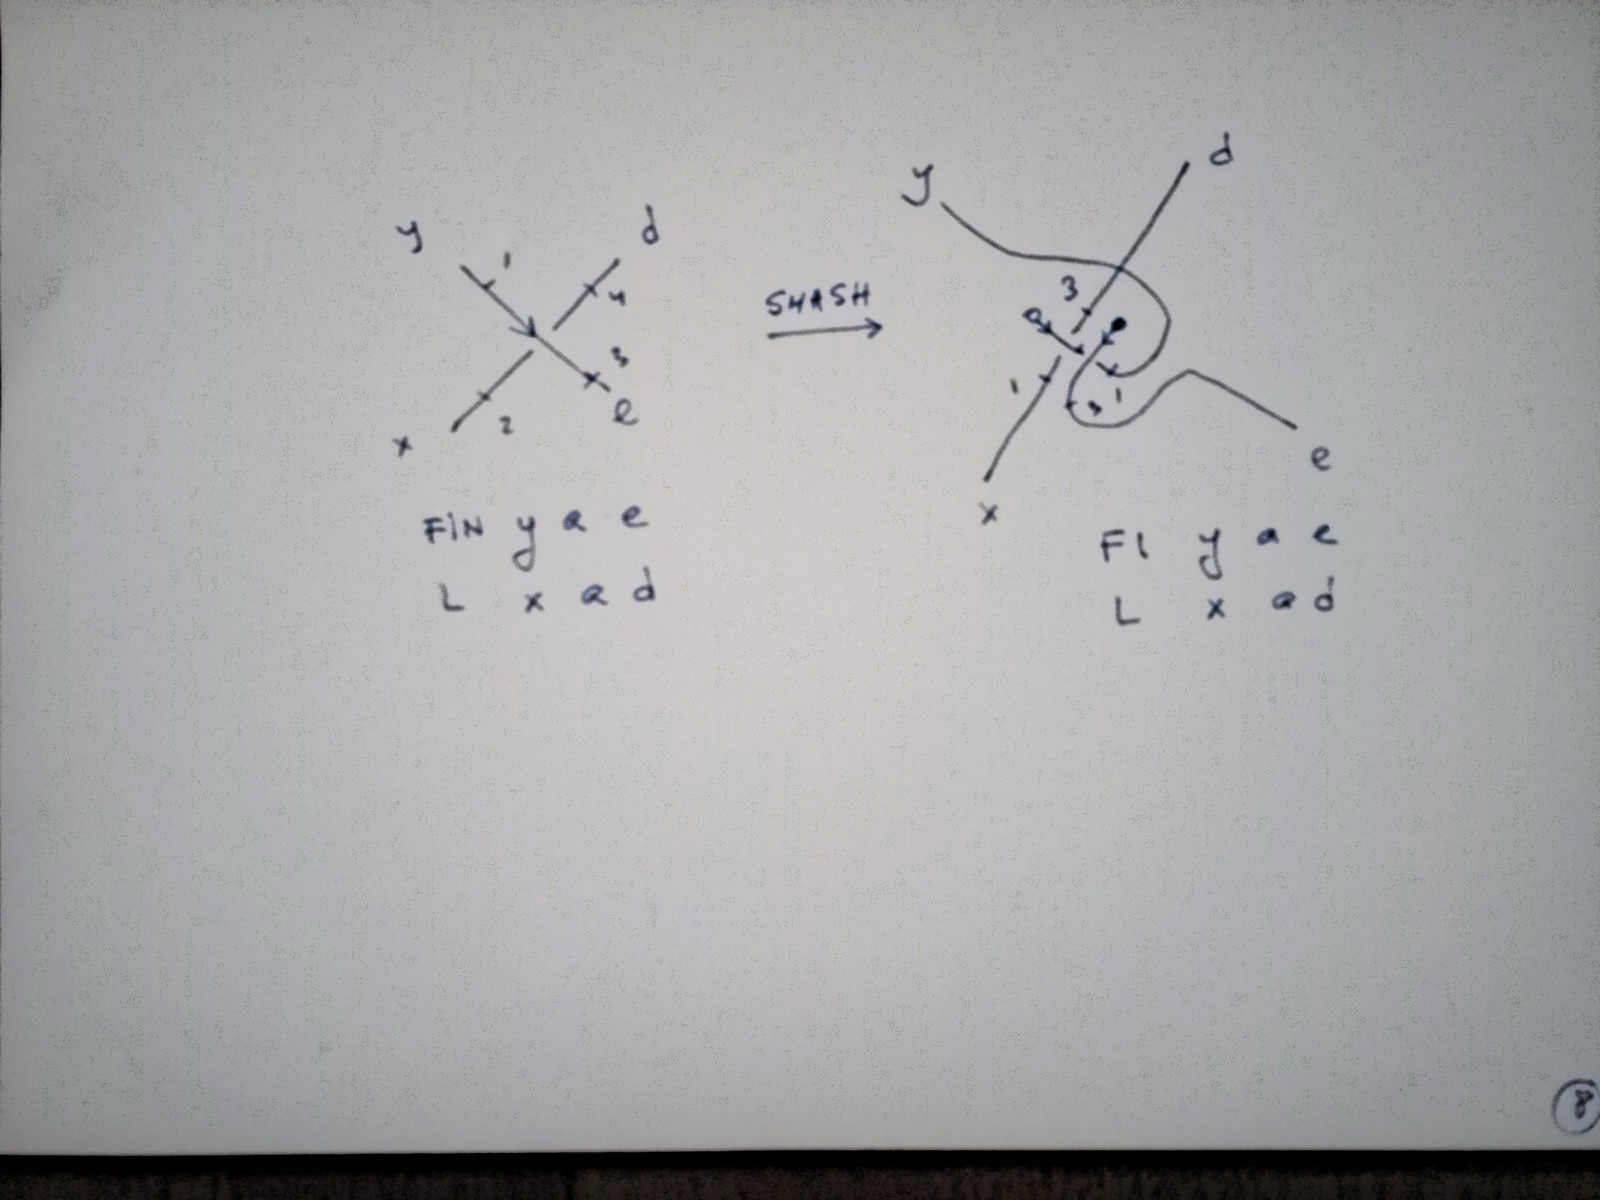
\includegraphics[width=0.75\linewidth]{img/3833.jpg}
\caption{The first smash rewrite}
\label{The-first-smash-rewrite}
\end{figure}

We see that, in the mol notation, it turns a FIN fanin into a FI 3
valent node, in the presence of a L node. Conversely, a pair of
half-zippers (black and white) connected as shown, turns into a
crossing.

The second smash rewrite, Figure \ref{The-second-smash-rewrite}, involves the other pair of black and white
half-zippers.

\begin{figure}[h!]
\centering
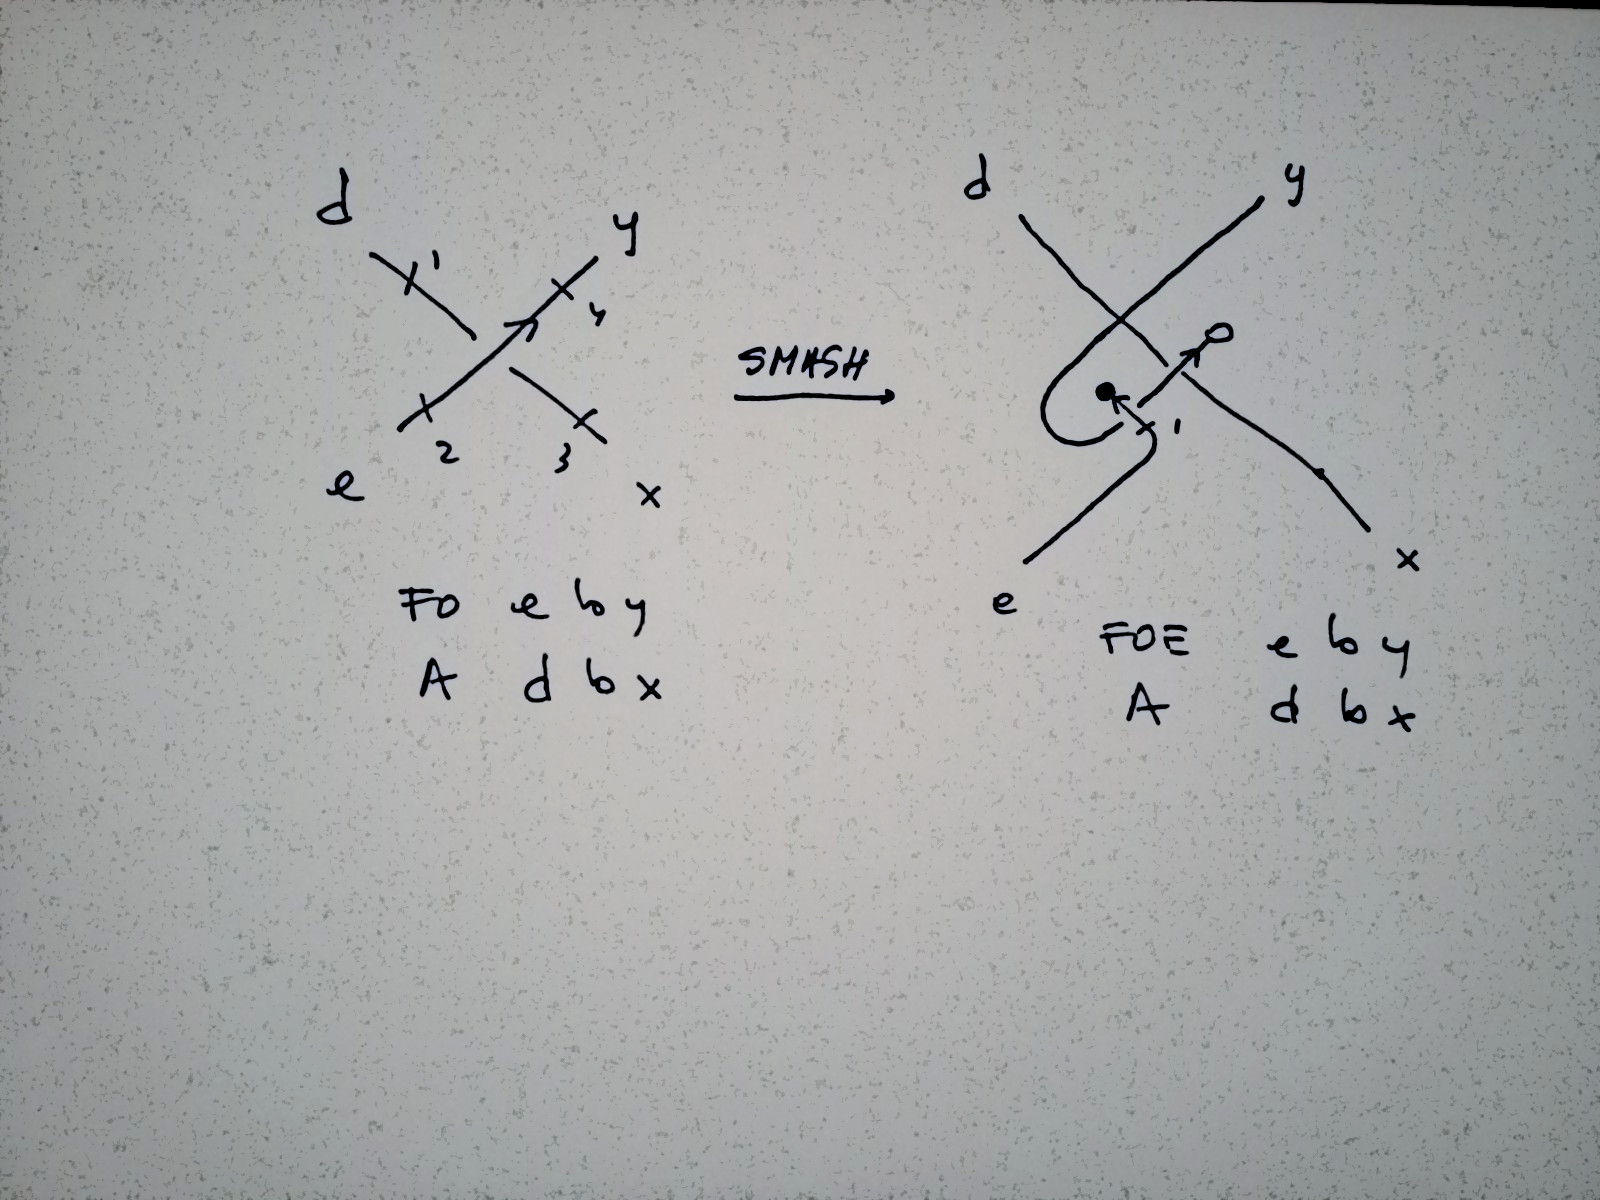
\includegraphics[width=0.75\linewidth]{img/3843.jpg}
\caption{The second smash rewrite}
\label{The-second-smash-rewrite}
\end{figure}

Finally, we have the \textbf{crossings rewrites}! They are the R1, R2,
R3 familiar graph rewrites which involve only crossings.

In conclusion ZSS is a graph rewrite system which enlarges the
Reidemeister rewrites with supplimentary ones (zip, slip, smash) which
allow reconnection of edges, and tangle graphs with some 3 valent and 1
valent nodes.

ZSS is an improved version of \cite{buligazipper} 
\href{https://doi.org/10.6084/m9.figshare.1032660.v1}{Zipper logic
(figshare)} or \href{https://arxiv.org/abs/1405.6095}{arXiv:1405.6095
{[}math.CO{]}}.

Indeed, the original zipper logic used tangles with zippers, but there
were also fanins and fanout nodes. Here the fanins and fanouts are
embedded into crossings. Also, the duplication rewrites of zipper logic
are not local, in the sense that whole combinations of half-zippers
duplicate at once. Here we have rewrite duplications which are built
from more simple pieces.

As an example, in the Figure \ref{Duplication rewrite in ZSS} is described how we can achieve a duplication rewrite (L-FOE) in ZSS:

\begin{figure}[h!]
\centering
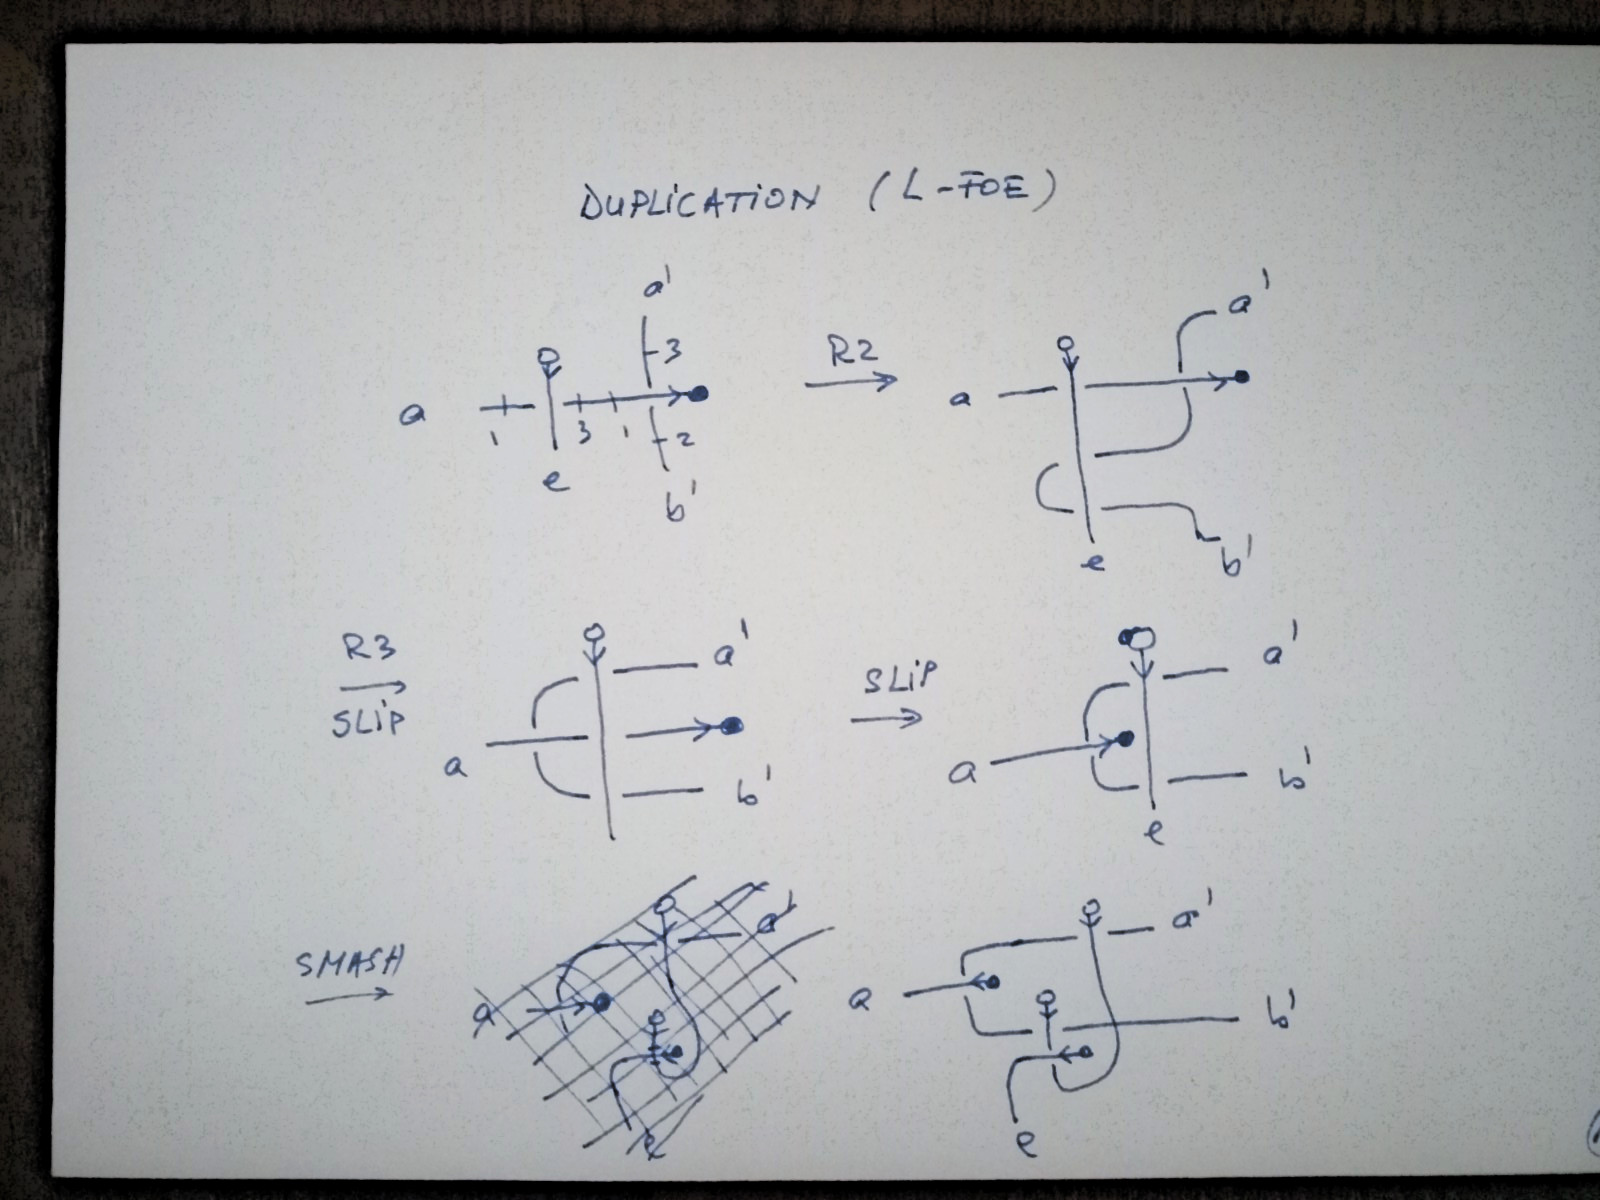
\includegraphics[width=0.75\linewidth]{img/3854.jpg}
\caption{Duplication rewrite in ZSS (here L-FOE)}
\label{Duplication rewrite in ZSS}
\end{figure}

We can give a similar proof of the duplication FI-A. Together
with the two zip rewrites and with the slip rewrites, we obtain all
rewrites of dirIC.

\textbf{Theorem.} ZSS is universal, because it implements directed
\href{https://mbuliga.github.io/quinegraphs/ic-vs-chem.html\#icvschem}{Interaction
Combinators (dirIC)}.

Recall that once we have the nodes L, FI, A, FOE and the mentioned
rewrites, then indeed we can reconstruct Lafont' Interaction combinators
by grouping A, L and FI, FOE, Figure \ref{Interaction-Combinators-and-dirIC}.

\begin{figure}[h!]
\centering
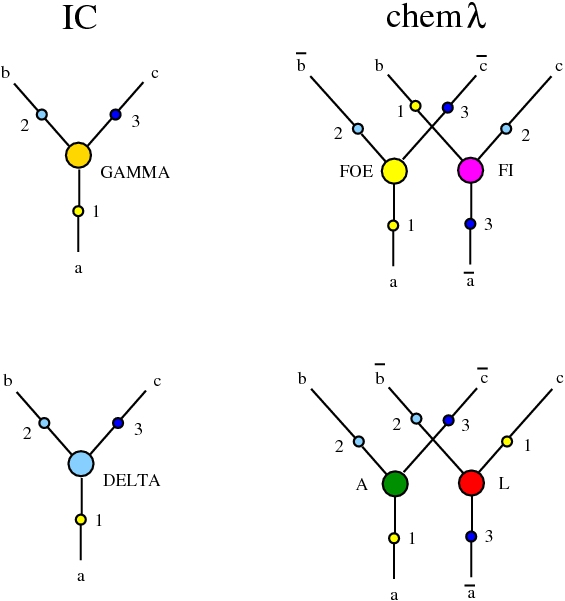
\includegraphics[width=0.6\linewidth]{img/dirIC.jpg}
\caption{Interaction Combinators and dirIC}
\label{Interaction-Combinators-and-dirIC}
\end{figure}

Not shown, the IC rewrites which delete nodes correspond to slip
rewrites in ZSS.

It is very interesting that in ZSS we obtain after smash rewrites pairs
of L, FI or A,FOE nodes. Compare with the groupings L,A or FI,FOE of
dirIC.

Moreover in ZSS we have the Reidemeister rewrites for crossings, which
are really useful, as shown in the L-FOE rewrite, which is obtained from
R2, R3, slip and smash rewrites.

\hypertarget{questions}{%
\subsection{Questions}\label{questions}}

\begin{itemize}
\item
  How can we add a passage to the limit like in emergent algebras?
\item
  How is this compatible with Pure See?
\item
  Is smash a rewrite which represents a measurement, if we were to try
  to use ZSS for quantum computing?
\end{itemize}



\begin{thebibliography}{99}

\bibitem{bawden}  A. Bawden,  Implementing Distributed Systems Using Linear Naming,  \href{https://dspace.mit.edu/handle/1721.1/7085}{A.I. Technical Report No. 1627}, MIT, (1993)

\bibitem{buligazipper} M. Buliga, Zipper logic, \href{https://doi.org/10.6084/m9.figshare.1032660.v1}{doi:0.6084/m9.figshare.1032660.v1}, \href{https://arxiv.org/abs/1405.6095}{arXiv:1405.6095} 

\bibitem{buligairq} M. Buliga, Emergent algebras, \href{https://arxiv.org/abs/0907.1520}{arXiv:0907.1520}

\bibitem{buligatangle} M. Buliga, Computing with space: a tangle formalism for chora and difference, \href{https://arxiv.org/abs/1103.6007}{arXiv:1103.6007}

\bibitem{buligacolin} M. Buliga, \href{https://mbuliga.github.io/colin/colin.pdf}{A problem in
emergent algebras}

\bibitem{buligaem} M. Buliga, The em-convex rewrite system, \href{https://arxiv.org/abs/1807.02058}{arXiv:1807.02058}

\bibitem{buligageneral} M. Buliga, Artificial chemistry experiments with chemlambda, lambda calculus, interaction combinators, 
\href{https://arxiv.org/abs/2003.14332}{arXiv:2003.14332}

\bibitem{chemlambda}  M. Buliga, \href{https://mbuliga.github.io/quinegraphs/history-of-chemlambda.html}{Graph rewrites, from emergent algebras to chemlambda}, \href{https://arxiv.org/abs/2007.10288}{arXiv:2007.10288}

\bibitem{carter} J.S. Carter, S. Kamada, M. Saito, Geometric Interpretations of Quandle Homology, \href{https://arxiv.org/abs/math/0006115v1}{arXiv:math/0006115v1}


\bibitem{zx} B. Coecke, R. Duncan, Interacting quantum observables: Categorical Algebra and Diagrammatics, \href{https://dx.doi.org/10.1088/1367-2630/13/4/043016}{doi:10.1088/1367-2630/13/4/043016}, \href{https://arxiv.org/abs/0906.4725}{arXiv:0906.4725}

\bibitem{lafont}  Y.  Lafont,  \href{https://pdfs.semanticscholar.org/6cfe/09aa6e5da6ce98077b7a048cb1badd78cc76.pdf}{Interaction
Combinators}, {\it Information  and  Computation} {\bf 137},  1,  69-101, (1997)


\end{thebibliography}

\end{document}
